\documentclass[a4paper,11pt]{article}

\usepackage{amsmath}
\usepackage[pages=some,scale=1,angle=0,opacity=1]{background}
\usepackage{bm}
\usepackage{caption}
\usepackage{colortbl}
\usepackage{enumitem}
\usepackage{eurosym}
\usepackage{fancyhdr}
\usepackage{geometry}
\usepackage{graphicx}
\usepackage{lineno}
\usepackage{mathtools}
\usepackage{multicol}
\usepackage{multirow}
\usepackage{parskip}
\usepackage{setspace}
\usepackage{ragged2e}
\usepackage{subcaption}
\usepackage{tabularx}
\usepackage{tabulary}
\usepackage{titlesec}
\usepackage[T1]{fontenc}
\usepackage{times}
\usepackage{url}
\usepackage{wallpaper}
\usepackage{wrapfig}
\usepackage{xcolor}

\usepackage[colorinlistoftodos]{todonotes}

\usepackage{array}
\newcolumntype{C}[1]{>{\centering\arraybackslash}p{#1}}

\newcommand\BackImage[2][scale=1]{%
\BgThispage
\backgroundsetup{
  contents={\includegraphics[#1]{#2}}
  }
}

% Shrink the spacing between references in the bibliography
%\usepackage{etoolbox}
%\patchcmd\thebibliography
% {\labelsep}
% {\labelsep\itemsep=-8pt\relax}
% {}
% {\typeout{Couldn't patch the command}}
 %%% End of code to add %%%

\bibliographystyle{h-physrev}

\renewcommand{\thesection}{\Alph{section}}

\newcounter{bar}
\newcommand{\taskcounter}{%
        \stepcounter{bar}%
        \thebar}

\setlist[itemize]{itemsep=-4pt, topsep=-2pt}

\usepackage{hyperref}
% \usepackage{cleveref}

\hypersetup{ colorlinks=false,
		     linkcolor=green,
		     urlbordercolor=blue,
		     pdfborderstyle={/S/U/W 1}}

\geometry{tmargin=2.5cm, bmargin=1.5cm, lmargin=2.cm, rmargin=2.cm}

\singlespacing
%\setstretch{1.035}

%\linenumbers

\setlength{\headheight}{15pt} 

\footskip=22pt
\headsep=18pt

\titlespacing*{\section}{0pt}{1pt}{1pt}
\titlespacing*{\subsection}{0pt}{1pt}{1pt}


%%%%%%%%%%%%%%%%%%%%%%%%%%%%%%%%%%%%%%%%%%%%%%%%
%%%%%%%%%%%%%%%%%%%%%%%%%%%%%%%%%%%%%%%%%%%%%%%%
\begin{document}
%%%%%%%%%%%%%%%%%%%%%%%%%%%%%%%%%%%%%%%%%%%%%%%%
%%%%%%%%%%%%%%%%%%%%%%%%%%%%%%%%%%%%%%%%%%%%%%%%

\renewcommand{\headrulewidth}{0pt}

\pagestyle{fancyplain}

% \lhead[\it Koskinen]{\it Koskinen}
% \chead{B2 - Scientific Proposal}
% \rhead{NuUnity}

\centerline{\huge ERC Starting Grant 2021}
\centerline{\huge Part B2}
% \centerline{\huge \textbf{Neutrino Probes of Non-Unitarity}}
% \centerline{\huge \textbf{in Particle Physics}}
% \centerline{\Large \textbf{(NuUnity)}}

\vspace{0.5cm}
%
%\ThisURCornerWallPaper{0.2}{plots/NeutrinoTriangleSimple.pdf}
%
%\makebox[50pt][l]{%
 % \raisebox{-\totalheight}[0pt][0pt]{%
  %  \includegraphics[width=4in]{plots/NeutrinoTriangleSimple.pdf}}}%
  
% \BackImage[width=0.07\textwidth]{plots/NeutrinoTriangleSimple.pdf}

% ------------------------------------------------------------------------------
% ------------------------------------------------------------------------------
% ------------------------------------------------------------------------------

% \section{Notes}
% \vspace{0.1 cm}

% \begin{itemize}
%     \item Comment that the whole project is risky given the potential for QG signals to be unmeasurably tiny (e.g. fr from guaranteed results), but the reward for  detection is huge and the fact I can rue out some models is a rare opportunity
%     \item Extra collaborative stuff like run workshops, collaborate with KM3NeT, open sourec signal code, etc
%     \item Synergy between event generator and (anti)neutrino separation, since both need detailed understanding of inelasticity
% \end{itemize}

% \textbf{14 PAGE LIMIT}

% ------------------------------------------------------------------------------
% ------------------------------------------------------------------------------
% ------------------------------------------------------------------------------

\todo{Generally need more specifics and more focus on experts}
\todo{Remove names (Jason, Troels, Marus, etc)?}

\section{State-of-the-art and Objectives}
\vspace{0.1 cm}

% \textbf{From instructions:} State-of-the-art and objectives. Specify the proposal objectives in the context of the state
% of the art in the research field. It should be clear how and why the proposed work is important for
% the field, and what impact it will have if successful, such as how it may open up new horizons or
% opportunities for science, technology or scholarship. Specify any particularly challenging or
% unconventional aspects of the proposal, including multi- or inter-disciplinary aspects.

\subsection{Introduction}

Despite every other force in Nature being successfully described by quantum mechanics, despite decades of theoretical efforts there is currently no quantum theory of gravity. A major contributing factor to this impasse is the paucity of meaningful experimental constraints to guide theory, a consequence of the astounding weakness of gravity compared to the other forces. In fact, gravity is only expected to become strong in particle interactions at energies 15 orders of magnitude higher than can be achieved in the most powerful particle colliders.

Even considering gravity's weakness as a fundamental force, there is hope to confront this glaring theoretical void in our understanding of the Universe. Neutrinos, ghost-like particles that are barely affected by the other forces of Nature, can travel vast distances, allowing even the very weak gravitational effects expected in a quantum theory of gravity to accumulate into potentially measurable signals. Furthermore, the bombardment of the Earth by cosmic rays from violent astrophysical sources produces an atmospheric neutrino flux with energies far exceeding those from man-made accelerators, allowing the suppression of the effects of quantum gravity to be at least partially overcome.

A quantum theory of gravity is expected to fundamentally alter the structure of space-time at microscopic distances, resulting in the degradation of the quantum superposition phenomenon of neutrino oscillations in a process known as neutrino decoherence. Additionally, symmetries fundamental to our current understanding of of particle physics such as $CPT$ symmetry may be violated if gravity is a quantum force, producing differences in neutrino oscillation effects between neutrinos and their antimatter counterparts. 

\begin{wrapfigure}{r}{0.45\textwidth} %this figure will be at the right
    \centering
		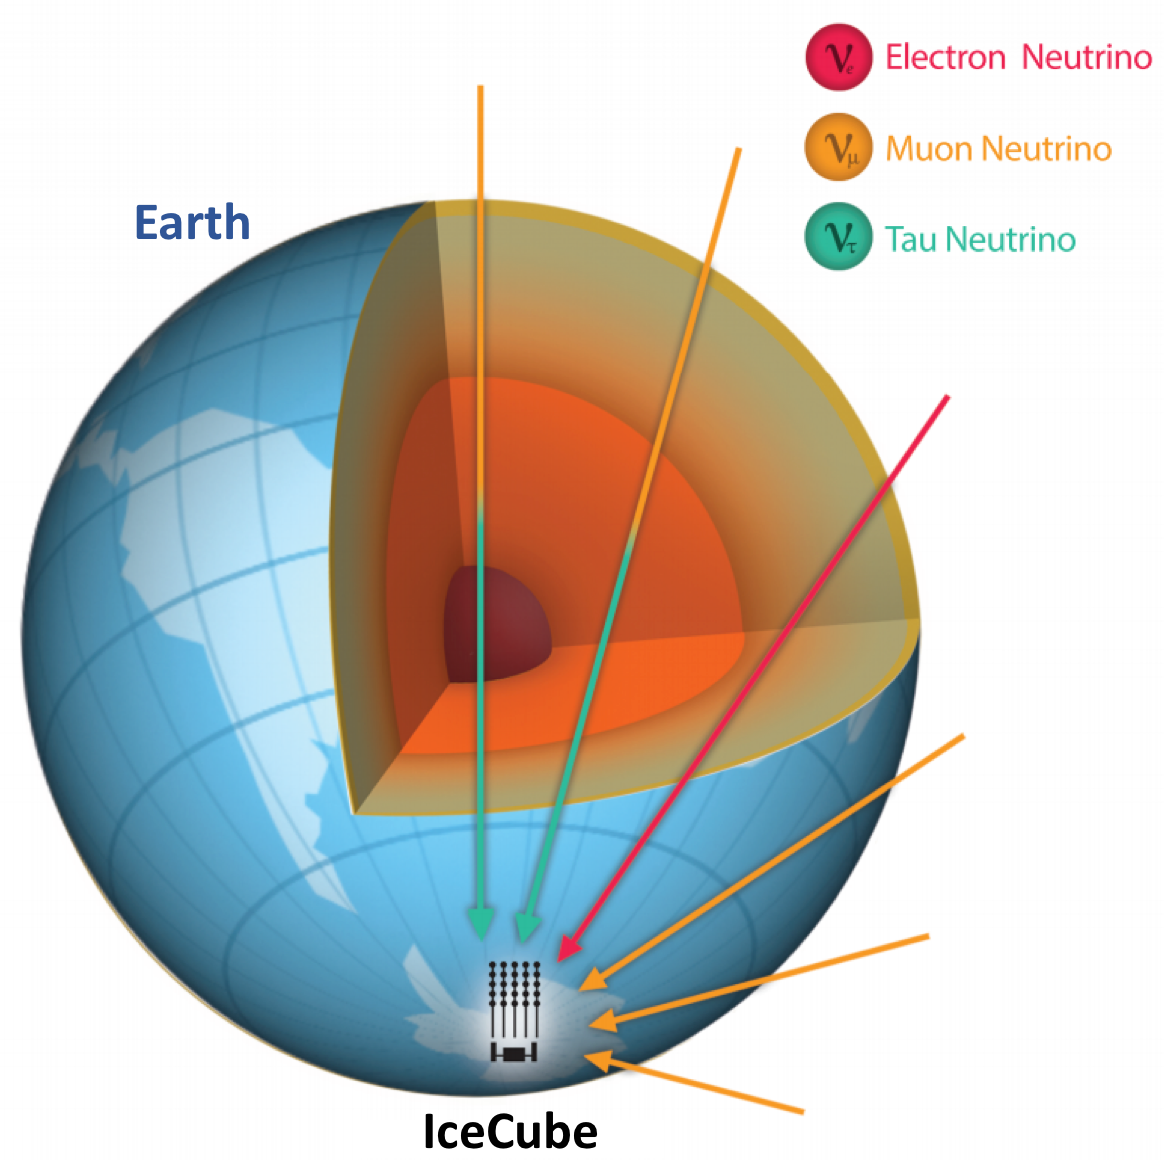
\includegraphics[width=1.\linewidth]{images/atmo_osc.png}
		\caption{Neutrinos produced in the atmosphere cross the Earth before detection in IceCube, oscillating and potentially experiencing the influence of quantum gravity as they propagate.}
		\vspace{-7pt}
		\label{fig:osc}
\end{wrapfigure}

My scientific vision is to perform the world's most sensitive searches for these signatures of quantum gravity with neutrinos, some of which will be world-firsts based on theoretical models I have developed. To do so I will exploit the vast flux of neutrinos produced in the Earth's atmosphere, observed using the world's largest and most sensitive neutrino telescope, the IceCube neutrino observatory at the South Pole. Crucially, I have demonstrated that these analyses are capable of detecting the predicted size of these quantum gravity effects in a number of scenarios, giving the realistic possibility of the first experimental detection of the signs of quantum gravity, which would be a truly revolutionary result. These results will also directly confront the question of why the Universe is dominated by matter rather than antimatter, one of the greatest open questions in physics.

I am both highly active in the theoretical modeling of the influence of quantum gravity on neutrino oscillations and also an experienced neutrino oscillation experimental data analyst, making me uniquely capable to tackle these ambitious searches for quantum gravity signals in neutrinos. On my own initiative I have developed models of neutrino decoherence resulting from quantum gravity that I will test in this project, enabling the inference of the underlying space-time properties from neutrino observations for the first time, and have a fast growing reputation in the theoretical community (recently being invited to co-author an international review of the field). As the leader of the recent generation of world-leading IceCube neutrino oscillation measurements (with a team of 13 physicists from 7 institutes in Europe and the US) I have experience leading a major international research project, and play a leading role in the IceCube detector upgrade that this project will utilise. My scientific leadership skills have been recognised by the IceCube collaboration, where I hold the roles of \textit{IceCube Upgrade simulation manager} (I am the named responsible person to the US National Science Foundation for delivering all simulations for this \$37 million project) and \textit{IceCube oscillation physics co-convener}. The window on quantum gravity this project will open is the result of my own physics vision, and I am ready to lead my own independent research group to realise these ambitious and potentially revolutionary measurements. \\

%\textbf{normally considered beyond the reach of experiment}.

% One of the greatest challenges in modern physics is the unification of gravity with the other forces of the Standard Model, but despite decades of efforts \textbf{no accepted quantum theory of gravity has been found}. This is in part due to the lack of experimental data to guide theorists, as the astounding weakness of gravity means that the effects of quantum gravity are only expected to become large at the Planck-scale, meaning vast energies ($10^{19}$\,GeV, 15 orders of magnitude more energetic than the most powerful particle colliders) or minuscule distances ($10^{-35}$\,m), which cannot be directly accessed by current or foreseeable experiments.

% However, there is hope. Neutrinos, ghost-like particle that barely interact with matter, can travel vast distances (even the entire Universe), allowing even the weak effects of quantum gravity to accumulate into potentially observable signals, and the extremely high energies of neutrinos from cosmic sources can partially overcome the suppression of Planck-scale physics at everyday energies. Furthermore, the fundamental changes to the microscopic nature of space-time expected in a quantum theory of gravity may disrupt the macroscopic quantum superposition phenomenon of neutrino oscillations, resulting in \textbf{neutrino decoherence} - the damping of neutrino oscillations in stochastic backgrounds - or \textbf{differences in the oscillation properties of neutrinos and antineutrinos} (their antimatter counterparts).

% \textit{coherent} nature of neutrino propagation would be disrupted by the fluctuating nature of quantum gravity, resulting in the observable phenomenon of \textbf{neutrino decoherence}; the damping of neutrino oscillations in stochastic backgrounds (the neutrinos act as a tiny quantum interferometers). 

% In this project I will perform the world's most sensitive and comprehensive search for these phenomena with the goal of detecting the first experimental sign of quantum gravity, using the high-energy, high-statistics neutrino data from the IceCube neutrino observatory. Crucially and almost uniquely, I have demonstrated that this project will achieve sensitivity to (and in some cases beyond) Planck-scale physics, which is \textbf{normally considered beyond the reach of experiment}. 

%I will perform model-independent searches, I will also test a number of specific models of the influence of quantum gravity on neutrino propagation that I have developed.

% I am perfectly placed to perform these measurements. I am internationally renowned expert in neutrino oscillation data analysis and leader of the most recent generation of world-leading IceCube oscillation measurements, am co-convener of IceCube oscillation physics, and play a leading role in the ongoing IceCube detector upgrade that this project will utilise. Furthermore, I am increasingly focusing on the power of neutrino oscillations to probe quantum gravity, and on my own initiative have developed detailed phenomenological models of the influence of quantum gravity on neutrinos that I will test in this project, demonstrating clear research independence, and have a growing reputation in the quantum gravity community (including recently being invited to co-author a review of the field). This project will also propel me into new territory as a researcher, studying high-energy regimes and astrophysical neutrino and gamma-ray data for the first time.% My work on decoherence and its connections to quantum gravity are entirely the result my own initiative, demonstrating clear research independence that I will take to new levels in this project, cementing my international profile as an expert in oscillation and new physics measurements with neutrinos.


\subsection{Quantum gravity}

% \begin{wrapfigure}{r}{0.43\textwidth} %this figure will be at the right
%     \centering
%         % \vspace{-9pt}
%         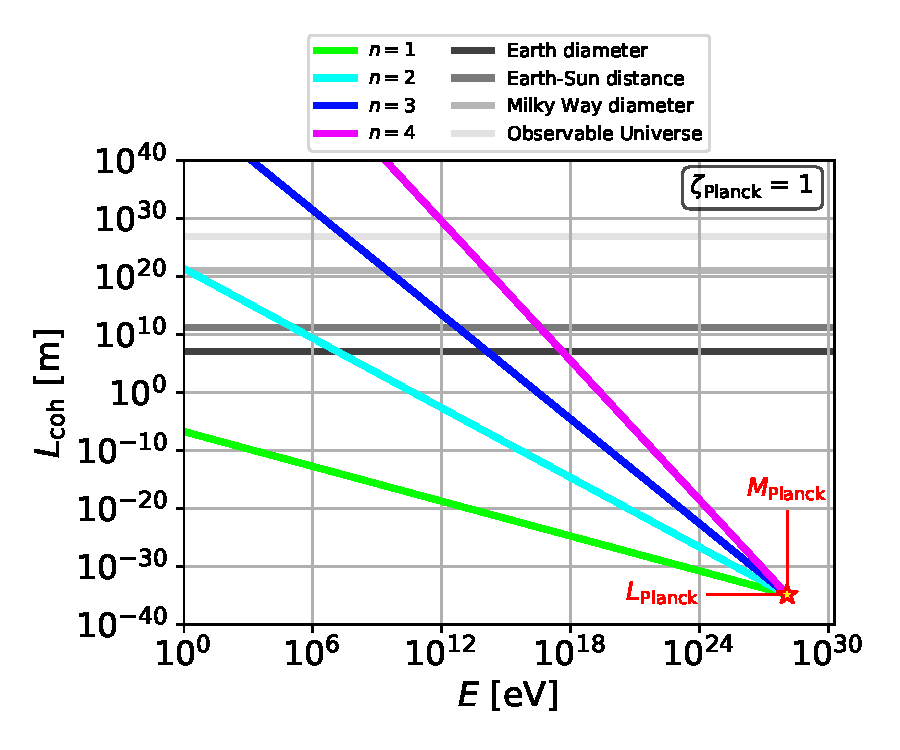
\includegraphics[trim=0.0cm 0.4cm 0.cm 0.5cm, clip=true, width=1.\linewidth]{images/paper_plots_coherence_length_vs_energy_planck.pdf}
% 		\caption{Distance at which decoherence due to Planck-scale physics is expected to become significant, for a variety of power-law, $E^n$, energy dependencies~\cite{PhysRevD.102.115003}. Sensitivity can be achieved with terrestrial neutrino sources in some scenarios, whilst astrophysical distances are required in others.}
% % 		\vspace{-7pt}
% 		\label{fig:planck_scale_coherence_length}
% \end{wrapfigure}

\begin{wrapfigure}{r}{0.5\textwidth} %this figure will be at the right
    \centering
		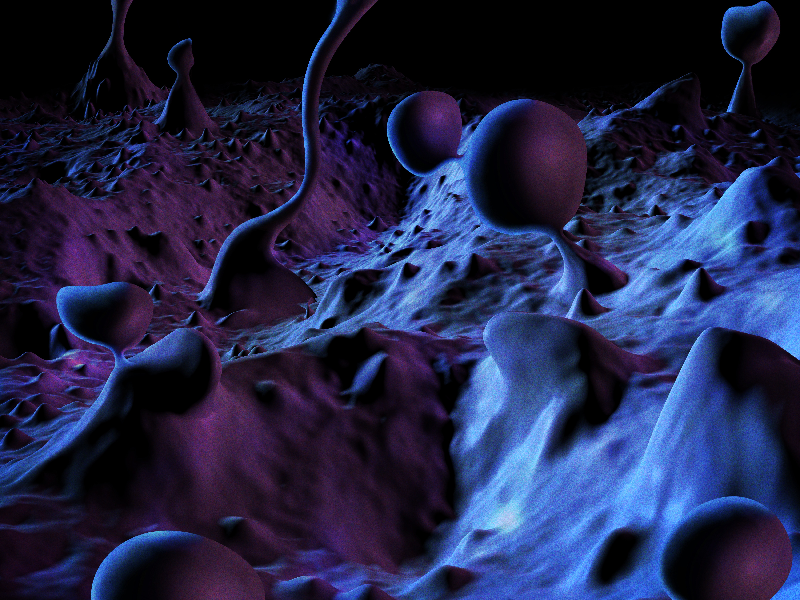
\includegraphics[width=1.\linewidth]{images/quantum_foam_2.png}
		\caption{An artists impression of the fluctuating nature of space-time at tiny distance scales, as expected in a quantum theory of gravity.}
		\vspace{-7pt}
		\label{fig:spacetime_foam}
\end{wrapfigure}

Einstein's theory of general relativity (GR) has been remarkably successful at describing the influence of gravity at macroscopic scales, but breaks down when applied to dense, small systems such as black holes and the early Universe\todo{More about why GR and QM are incompatible}, meaning GR cannot be a full story and a quantum theory of gravity must exist. The effects of quantum gravity are typically expected to be strong at the \textit{Planck scale}, meaning colossal energies of $10^{19}$ GeV or minuscule distances of $10^{-35}$ m, meaning these signals are likely suppressed at the energy and distance scales we can experimentally probe and have thus far evaded detection.

Although we do not have a complete quantum theory of gravity, we do know some of the features it is expected to exhibit. Most notably, the fabric of space-time itself would be subject to the intrinsic uncertainty present in all quantum theories and fluctuate at tiny distance scales~\cite{PhysRev.97.511, Hawking} (see Fig. \ref{fig:spacetime_foam}). This is far cry from the smooth, flat picture of space-time we are familiar with in the macroscopic world described by GR. 

The most straightforward consequence of this are so-called \textit{lightcone fluctuations}~\cite{PauliLightcone, Ford1999, gr-qc/9909085}, where the fluctuating space-time curvature causes variations in the time taken by a particle to travel between two points. Though these fluctuations would be very small, their effects could accumulate over large distances into measurable effects. Neutrinos propagating in this fluctuating space-time would become increasingly out of phase with each other.

It is also predicted that these space-time fluctuations manifest as so-called \textit{virtual black holes} (VBH)~\cite{Hawking1982,PhysRevD.53.3099}, which are microscopic black holes that form in the vacuum and promptly evaporate. Whilst exotic sounding, this is simply the gravitational analogue of the virtual electron pairs that are integral to our modern understanding of electromagnetism. A neutrino encountering a VBH would undergo severe modifications to its propagation, with global symmetries potentially violated in the interaction~\cite{Anchordoqui:2005gj, PhysRevD.102.115003, Hellmann:2021jyz}. This could result in neutrino flavour violations, conversions to different particle types altogether or even the loss of the neutrino from the observable Universe altogether.

A broad range of experimental tests of quantum gravity have been performed, ranging from high precision photon interferometry laboratory experiments (REFs) to astrophysical observations of cosmic messenger particles such as $\gamma$-rays and gravitational waves from distant sources (REFs). There have also been experimental tests for the features predicted by some of the leading theories seeking to describe quantum gravity, such as the additional space-time dimensions predicted by string/brane theories (REFs), or violations of Lorentz inveriance, $CPT$ symmetry or the weak equivalence principal (REFs). No signal of quantum gravity has been detected thus far however despite our knowledge that such a theory must exist, and without an accepted theory to guide us it is essential to perform the broadest range of tests possible and seek to continually increases sensitivity to these suppressed effects. \\

% TODO neutrinos


% It is also often predicted that these fluctuations can collapse to form so-called `virtual black holes' (VBH)~\cite{Hawking1982,PhysRevD.53.3099}, which are minuscule and quickly evaporate. Whilst this sounds exotic, it is in fact simply the gravitational analogue of the virtual electron-positron pairs that are fundamental to our understanding of the electromagnetic force. A neutrino encountering a VBH would likely experience significant disruption and/or loss of quantum information~\cite{hep-th/9508151}, resulting in decoherence. 



% Neutrinos travelling from source to detector thus become increasingly out of phase with each other.

% Though these fluctuations would be very small, their effects accumulate over large distances. It is also often predicted that these fluctuations can collapse to form so-called `virtual black holes' (VBH)~\cite{Hawking1982,PhysRevD.53.3099}, which are minuscule and quickly evaporate. Whilst this sounds exotic, it is in fact simply the gravitational analogue of the virtual electron-positron pairs that are fundamental to our understanding of the electromagnetic force. A neutrino encountering a VBH would likely experience significant disruption and/or loss of quantum information~\cite{hep-th/9508151}, resulting in decoherence. 

% Particle's propagating in this fluctuating space-time 

% In the absence of an accepted theory of quantum gravity, it is necessary to test many scenarios. A key feature expected in quantum gravity is that space-time itself is subject to the inherent uncertainty of quantum mechanics and fluctuates at very small distance scales~\cite{misner1973gravitation}. This is precisely the kind of stochastic environment that would produce neutrino decoherence~\cite{Mavromatos_2009,PhysRevD.102.115003}. %This project will exploit the unparalleled sensitivity of neutrinos to decoherence to search for both specific quantum gravity scenarios and a more general approach that is sensitive to decoherence effects from a broad range of sources. 

% The most straightforward such decoherence mechanisms are so-called `lightcone' fluctuations\cite{Ford1999, gr-qc/9909085}, where the fluctuating space-time curvature causes the travel distance/time between two points to fluctuate. Neutrinos travelling from source to detector thus become increasingly out of phase with each other, leading to decoherence. Though these fluctuations would be very small, their effects accumulate over large distances. It is also often predicted that these fluctuations can collapse to form so-called `virtual black holes' (VBH)~\cite{Hawking1982,PhysRevD.53.3099}, which are minuscule and quickly evaporate. Whilst this sounds exotic, it is in fact simply the gravitational analogue of the virtual electron-positron pairs that are fundamental to our understanding of the electromagnetic force. A neutrino encountering a VBH would likely experience significant disruption and/or loss of quantum information~\cite{hep-th/9508151}, resulting in decoherence. 

% % A stronger, highly promising signal occurs if these fluctuations sufficiently curve space-time sufficiently in a miniscule volume to collapse and form a singularity, creating a microscopic `virtual black hole' (VBH) which quickly evaporates (analogous to the well known virtual electron-positron pairs of the electromagnetic force). A neutrino encountering a VBH would likely experience significant wavefunction disruption and/or the loss of quantum information~\cite{hep-th/9508151}, which I have shown can produce observable effects even if only a small fraction of detected neutrinos experience such an event. 

% % , which I have shown can produce observable effects even if only a small fraction of detected neutrinos experience such an event.

% I have developed a phenomenological model of the influence of neutrino-VBH ($\nu$-VBH) interactions on neutrino propagation in a range of well motivated scenarios~\cite{PhysRevD.102.115003}, and remarkably have demonstrated that \textbf{sensitivity to Planck-scale physics can be achieved using the high-energy neutrinos detected by the IceCube neutrino observatory} (see Fig. \ref{fig:planck_scale_coherence_length}), even if only a small fraction of neutrinos undergo these encounters. I have recently also developed a model of neutrino decoherence from lightcone fluctuations\todo{Add referecnce once submitted} (submitted to PhysRevD), accounting for both fluctuating space-time curvature and also scenarios where the speed of light fluctuates for high energy particles  (so-called \textit{stochastic Lorentz invariance violation}~\cite{Vasileiou2015}). I will perform stringent experimental tests of these models in this project.

\subsection{Neutrino oscillations and decoherence}

\begin{wrapfigure}{r}{0.42\textwidth} %this figure will be at the right
    \centering
		\vspace{-7pt}
		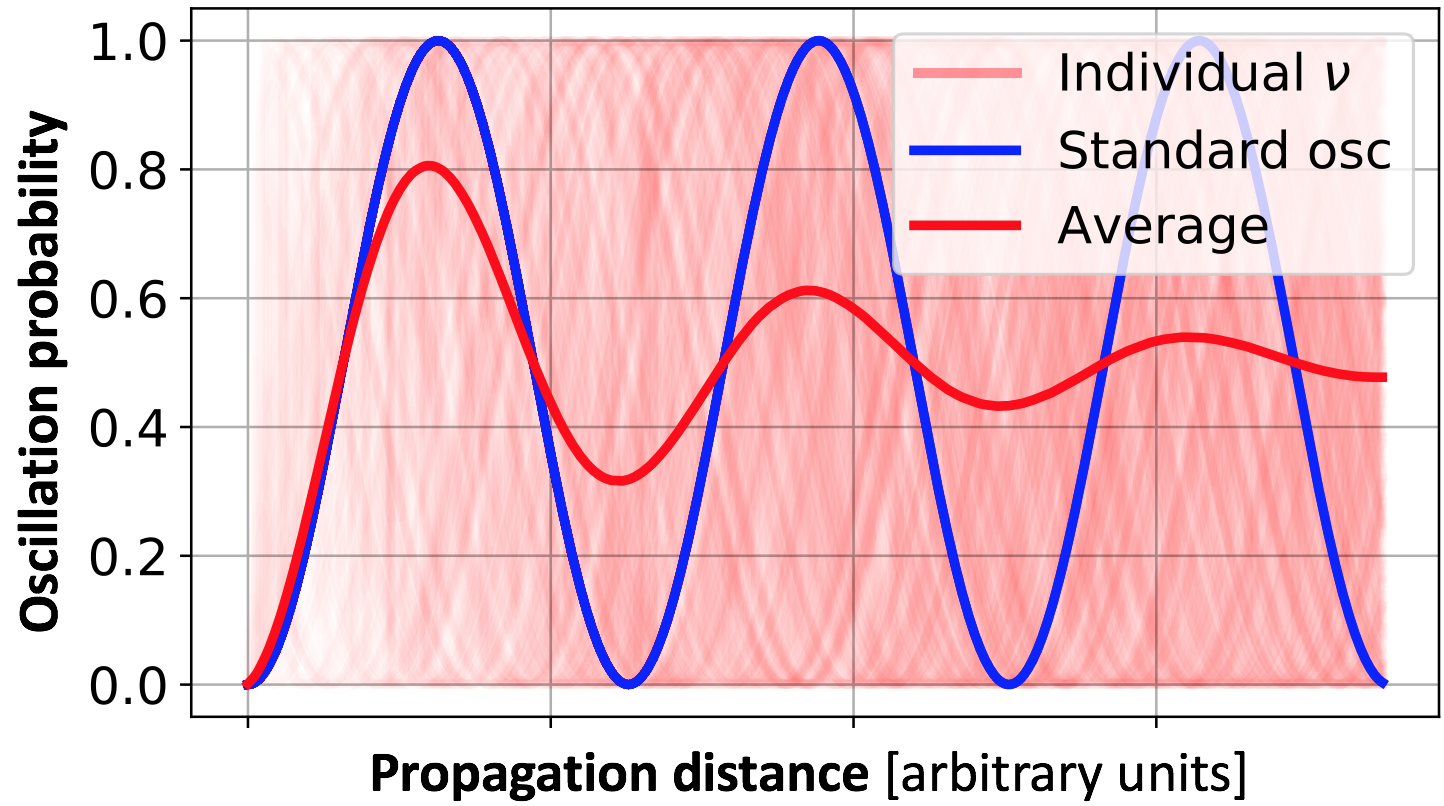
\includegraphics[width=1.\linewidth]{images/decoherence.png}
		\caption{Toy model example of individual neutrinos propagating in a fluctuating environment, which are perturbed and become increasingly out of phase, resulting in damping of the average oscillation probability.}
		\vspace{-5pt}
		\label{fig:decoherence}
\end{wrapfigure}

Neutrinos exhibit the peculiar phenomenon of \textit{neutrino oscillations} where a neutrino produced as one type (\textit{flavour}) may be detected later as another~\cite{Fukuda:1998mi, Ahmad:2001an,Ahmad:2002jz}. The detection of these oscillations implies that neutrinos have non-zero (albeit tiny) masses, contrary to the Standard Model (SM) of particle physics, providing one of the only confirmed experimental signs of Beyond Standard Model (BSM) physics today, and the measurements of these oscillations is a major field of active research today.

However, the quantum superposition effect producing these oscillations would be disrupted for neutrinos propagating in fluctuating space-time, resulting in the damping of neutrino oscillations and averaging of neutrino flavors in a process known as neutrino decoherence~\cite{Benatti_2000, PhysRevLett.85.1166}. The oscillating nature of neutrinos and their ability to travel vast distances unperturbed by the other forces of nature makes them uniquely sensitive to decoherence effects from quantum gravity, with the neutrinos acting as tiny quantum interferometers. Decoherence measurements are potentially sensitive to a range of new physics scenarios (REFs - grab from signal modelling section), including those only accessible via the gravitational force (to which nearly all other particle physics measurements are essentially blind)~\cite{Hellmann:2021jyz}.

I have developed phenomenological models of the influence of neutrino-VBH ($\nu$-VBH) interactions on neutrino propagation in a range of scenarios~\cite{PhysRevD.102.115003}, and remarkably have demonstrated that the resulting damping effect from \textit{natural} Planck scale physics can be resolved using neutrino oscillation measurements by the IceCube neutrino observatory, even if only a small fraction of neutrinos undergo these encounters. More recently I have also developed a model of neutrino decoherence resulting from lightcone fluctuations~\cite{2103.15313} (submitted to the journal \textit{Phys. Rev. D}), accounting for both fluctuating space-time and also scenarios where the speed of light fluctuates for high energy particles (so-called \textit{stochastic Lorentz invariance violation}~\cite{Vasileiou2015}), yielding further potential signals in IceCube data. These models are the first to directly connect the potentially observable phenomenology of neutrino decoherence to the underlying microphysics of a quantum theory of gravity, allowing experimental constraints on the fundamental nature of space-time to be made for the first time in this project. .

\textbf{State-of-the-art:} Neutrino decoherence searches have been performed using data from nuclear reactors, the Sun, the Earth's atmosphere and particle accelerators (generally with simple mathematical expressions rather than specific models), with no signal observed thus far. Despite the large distances travelled, neutrinos of extragalactic origin are not in general well suited to decoherence searches due to the incoherent nature of the sources of these neutrinos~\cite{PhysRevD.102.115003}. Decoherence effects resulting from quantum gravity are expected to be energy-suppressed, and the strongest constraints to these signals to date were set using low statistics publicly released IceCube data (by non-collaboration authors). The measurements I will perform will exceed the sensitivity of these results by orders of magnitude, measure new strongly energy-suppressed (cubic and quartic) scenarios that have not previously been experimentally tested, test an unprecedented range of specific models, and include a robust treatment of systematic uncertainties not present in previous works, representing  major leap forward in this exciting field. \\

\todo{Proton decay}
\todo{GRB lightcone}
\todo{Lightcone holographic}

% \noindent \textbf{State-of-the-art:} High er E and longer baseline at LBL.

%I will perform stringent experimental tests of these models in this project.

%Decoherence is highly suppressed and as yet unoberved for neutrinos

% oscillations are coherent, meaning that the states of neutrinos of the same energy travelling the same path will evolve identically. This would be disrupted however if neutrinos couple to a stochastic environment in a process known as decoherence, observable as the \textbf{damping of neutrino oscillations} over distance (see Fig. \ref{fig:decoherence}). Decoherence is known in other quantum systems, but is highly suppressed and as yet unobserved for neutrinos due to their extremely feeble interactions with other (known) particles isolating them from their environment.

% Neutrinos propagate as a superposition of three quantum states, giving rise to the peculiar phenomenon of \textit{neutrino oscillations} where a neutrino produced as one type (\textit{flavor}) may be detected later as another~\cite{Fukuda:1998mi, Ahmad:2001an,Ahmad:2002jz}. These oscillations are coherent, meaning that the states of neutrinos of the same energy travelling the same path will evolve identically. This would be disrupted however if neutrinos couple to a stochastic environment in a process known as decoherence, observable as the \textbf{damping of neutrino oscillations} over distance (see Fig. \ref{fig:decoherence}). Decoherence is known in other quantum systems, but is highly suppressed and as yet unobserved for neutrinos due to their extremely feeble interactions with other (known) particles isolating them from their environment.

% I have developed a phenomenological model of the influence of neutrino-VBH ($\nu$-VBH) interactions on neutrino propagation in a range of well motivated scenarios~\cite{PhysRevD.102.115003}, and remarkably have demonstrated that \textbf{sensitivity to Planck-scale physics can be achieved using the high-energy neutrinos detected by the IceCube neutrino observatory} (see Fig. \ref{fig:planck_scale_coherence_length}), even if only a small fraction of neutrinos undergo these encounters. I have recently also developed a model of neutrino decoherence from lightcone fluctuations\todo{Add referecnce once submitted} (submitted to PhysRevD), accounting for both fluctuating space-time curvature and also scenarios where the speed of light fluctuates for high energy particles  (so-called \textit{stochastic Lorentz invariance violation}~\cite{Vasileiou2015}). I will perform stringent experimental tests of these models in this project.

% Decoherence can result in a range of scenarios, including quantum gravity, neutrino interactions with Dark Matter~\cite{1909.11271, EPJC802020}, string theory~\cite{Ellis:1997jw,doi:10.1142/S0217732397000248,PhysRevD.80.124019,Mavromatos2010}, diffuse gravitational waves~\cite{Dvornikov_2020}, and can reveal whether neutrinos are their own antiparticle~\cite{CAPOLUPO2019298, 2001.07580}. Decoherence measurements can thus confront some of the biggest questions in particle physics.


\subsection{$CPT$ violation and matter-antimatter asymmetry}

\textbf{TODO Need a new $CPT$-V figure, keep it sensible rather than trying to motivated the full E range (decoherence does that already)}

% \begin{wrapfigure}{r}{0.43\textwidth} %this figure will be at the right
\begin{wrapfigure}{c}{0.43\textwidth} %this figure will be at the right
    \centering
    % \vspace{-9pt}
    \includegraphics[trim=0.0cm 0.0cm 0.cm 0.0cm, clip=true, width=1.\linewidth]{images/CPTv_IceCube.pdf}
	\caption{Difference between neutrino and antineutrino oscillation probability in the presence of $CPT$-V, showing potential signals that no experiment other than IceCube could detect. No difference is expected if $CPT$ is not violated, meaning any observed difference must result from new physics. }
% 	\vspace{-7pt}
	\label{fig:$CPT$v}
\end{wrapfigure}

Like other particles, neutrinos have antimatter counterparts known as antineutrinos, which have mirrored but otherwise identical properties. However, if gravity is a quantum force then the uncertain nature of space-time \todo{More specific here} can result in differing properties between matter and antimatter, known as \textbf{$CPT$ violation} ($CPT$-V)~\cite{Mavromatos:2005mi, AmelinoCamelia:2008qg, RalfLehnert:2016grl}. 

For neutrinos, $CPT$-V predicts \textbf{differing oscillation frequencies and amplitudes between neutrinos and antineutrinos} through differing mass splittings and mixing angles~\cite{Barenboim:2017ewj}, a potentially observable signal. These effects are likely suppressed at energies below the Planck scale, but this can be partially overcome in the high energy measurements of neutrino oscillations with IceCube (orders of magnitude higher in energy than any other experiment) to yield \textbf{sensitivity to signals to which all other experiments would be blind} (see Fig. \ref{fig:$CPT$v}). 

Detecting $CPT$-V would have profound consequences even beyond the search for quantum gravity. One of the biggest questions in physics is why the Universe appears to almost entirely consist of matter, and not antimatter, since (in the absence of $CPT$-V or other new physics) both are expected to have been produced equally~\cite{Sakharov_1991}. The very fact we are even here to ponder this question is a consequence of this, since without this imbalance all matter and antimatter would have annihilated to leave a Universe devoid of stars, planets or life. Known differences between matter/antimatter (so-called $CP$-violation) can only account for a tiny fraction of the observed imbalance, meaning that \textbf{new physics like $CPT$-V must exist}. The energy-suppressed $CPT$-V I will search for is an excellent candidate to explain this, as these effects would have been strong in the high temperatures of the early Universe when (anti)matter was forming~\cite{Mavromatos:2017cxr, hep-ph/9809542}. Beyond quantum gravity, $CPT$-V in neutrinos has also been predicted to result from interactions between neutrinos and Dark Matter (DM)~\cite{Capozzi:2018bps, 1904.02518}. Furthermore, tensions have emerged in neutrino vs antineutrino oscillation measurements~\cite{Abe:2019vii,NOvA_CP_result}, potentially indicating the presence of new physics that this project could reveal, making this measurement more important than ever.

\todo{More generally $CPT$-V from scattering on matter/backgrounds~\cite{Capolupo:2020myw}? Maybe motivate with the fact that standad matter effects are $CPT$ violating, and so $CPT$ effects from unknown backgrounds are well motivated.}

\noindent \textbf{State-of-the-art:} In the absence of a concrete model of quantum gravity (or other $CPT$-V theory) it is essential to probe the broadest possible range signals~\cite{hep-ph/9809542} for signs of $CPT$-V. Experimental constraints exist for neutral kaons (REFs), neutrinos~\cite{Adamson:2013whj, Ohlsson:2014cha}, hadron colliders~\cite{vanTilburg:2016awx} and in precision tests of low energy systems such as particle magnetic moment measurements (REFs) and (anti)hydrogen spectroscopy~\cite{Kostelecky:2015nma}, with no observed signal to date. This indicates that such effects are highly suppressed, as expected in a quantum theory of gravity.  The sensitivity of neutrino oscillations to very small masses (and thus small mass differences) makes them one of the best motivated search channels~\cite{PhysRevD.99.075022}, and the measurements in this work will test $CPT$-V at orders of magnitude higher energies that existing limits with accelerator neutrinos. Additionally, the precision of IceCube's neutrino oscillation measurements has reached parity with accelerator experiments for the first time (in an analysis I lead), and will surpass this with the data from the next-generation IceCube Upgrade. Coupled with pioneering (anti)neutrino separation methods I will develop, this project will afford unparalleled sensitivity to energy-suppressed $CPT$-V in neutrino oscillations. \\


% The concept of \textit{symmetries} in physics are fundamental to understanding of the microscopic world. 
% Charge-Parity-Time ($CPT$) symmetry - meaning that the physics of a system remains unchanged when simultaneously the charge flips, directions are mirrored and the direction of time reverses - is a cornerstone of the quantum field theories that have described our Universe at microscopic scales with unprecedented success. However, the fundamental conditions required for $CPT$ symmetry are not expected to hold in a quantum theory of gravity (for example due to the fluctuating nature of space-time), leading to the prediction that $CPT$ symmetry may be violated at some energy scale~\cite{Mavromatos:2005mi, RalfLehnert:2016grl}. An experimental signature of $CPT$ violation ($CPT$-V) would be a game changing result in the search for quantum gravity and more generally would shake the foundations of quantum field theories.

% A potential consequence of $CPT$-V is differing properties such as mass between particles and antiparticles, which for neutrinos would manifest as differing oscillations for neutrinos and antineutrinos~\cite{Ohlsson:2014cha, Barenboim:2017ewj}. Such effects have been probed with neutral kaons and neutrinos~\cite{TAKEUCHI201279, Adamson:2013whj}, but I have identified that the atmospheric neutrino oscillations observed by IceCube (orders of magnitude higher energy than any other experiment) are likely far more sensitive to such effects, given that $CPT$-V (and other effects of Planck scale physics) are expected to be suppressed at low energies. Fig. \ref{fig:$CPT$v} shows two example $CPT$-V scenarios (in an energy-dependent model I have developed) that produce significant effects for IceCube but would not have been detected by previous searches with accelerators, and I will perform the world's most sensitive search for energy-dependent $CPT$-V. 


% \todo{Another possible manifestation...}Additionally, potential $CPT$-V effects in neutrino decoherence have been identified~\cite{Mavromatos_2009, Barenboim:2004wu, Carrasco:2018sca}, providing a powerful synergy between the elements of this proposal. I have shown that such effects can produce potentially observable signals for high energy neutrinos in IceCube, and will also test these effects in this work. 


\subsection{The IceCube neutrino observatory and the IceCube Upgrade}

\begin{wrapfigure}{r}{0.45\textwidth} %this figure will be at the right
    \centering
	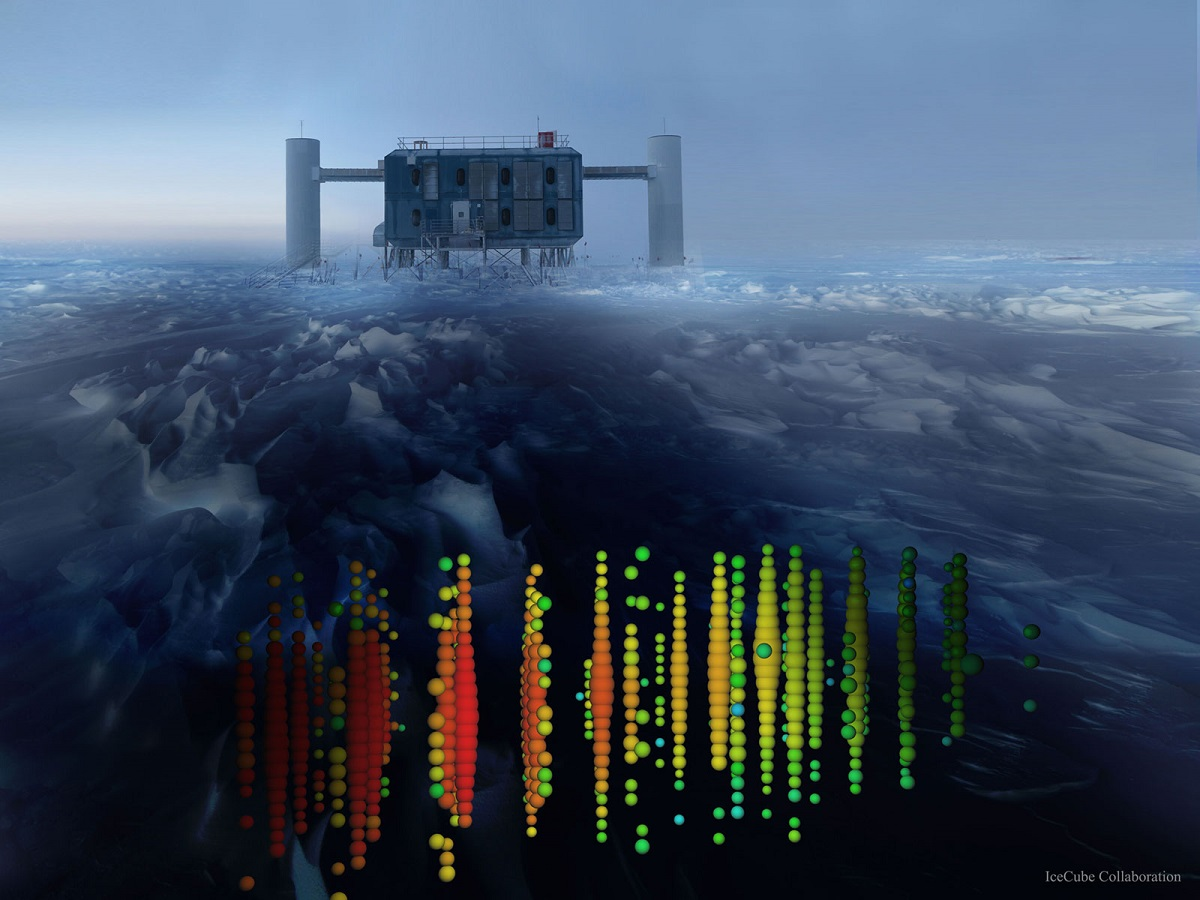
\includegraphics[width=1.\linewidth]{images/IceCube_1200x.jpg}
	\caption{The IceCube neutrino observatory at the South Pole. Cherekov light from neutrino interactions in the glacial ice deep below the surface are detected by PMTs.}
% 		\vspace{-7pt}
	\label{fig:atmo_osc}
\end{wrapfigure}

The IceCube neutrino observatory~\cite{Aartsen_2017}, located at the geographic South Pole, instruments a vast 1 billion tons of glacial ice deep below the surface with 5160 optical sensors, each containing a single photomultipier tube (PMT), to detect Cherenkov light produced by the interactions of neutrinos in the ice. This truly colossal 1 Gton detector detects huge numbers of neutrinos produced in air showers when cosmic rays slam into the Earth's atmosphere, many of which oscillate from muon to tau flavoured as they cross the Earth (Fig. \ref{fig:osc}), as well as neutrinos of extra-galactic origin. These neutrinos are detected across a staggering six orders of magnitude in energy (GeV to PeV), dwarfing the energy reach of even particle colliders. 

%These high-energy neutrinos with long travel distances are perfect to search for decoherence from Planck-scale physics, and the huge statistics allows even very weak effects to be probed (crucial for quantum gravity). 

\begin{wrapfigure}{c}{0.45\textwidth} %this figure will be at the right
    \centering
	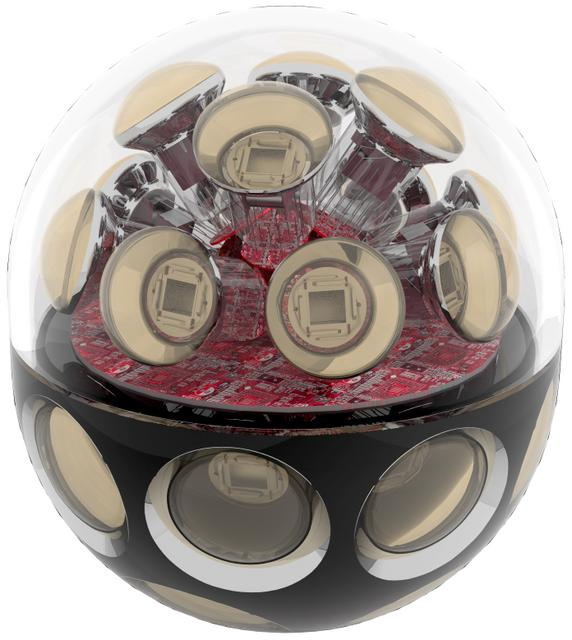
\includegraphics[width=1.\linewidth]{images/mdom.jpg}
	\caption{One of the new multi-PM optical modules to be installed in the IceCube Upgrade.}
% 		\vspace{-7pt}
	\label{fig:mDOM}
\end{wrapfigure}


Furthermore, in 2023-24 IceCube will be substantially upgraded~\cite{IceCubeUpgrade_ICRC2019} with sensitive new multi-PMT optical modules, dramatically increasing the instrumentation density in a 2 Mton core. I lead the international group conducting the simulation studies of the goals and performance of the IceCube Upgrade experiment~\cite{IceCubeUpgrade_ICRC2019, NuFactProceedings}, which show factor 2-4 improvements in detector efficiency and resolution, providing a truly next-generation precision neutrino physics facility. Additionally, a host of new calibration devices will be deployed to allow precise characterisation of the natural detection medium and significantly reduce systematic uncertainty.\\



% ------------------------------------------------------------------------------
% ------------------------------------------------------------------------------
% ------------------------------------------------------------------------------
% ------------------------------------------------------------------------------

\section{Methodology}
\vspace{0.1 cm}

\textbf{From instructions:} Describe the proposed methodology in detail including any key
intermediate goals. Explain and justify the methodology in relation to the state of the art, and
particularly novel or unconventional aspects addressing the 'high-risk/high-gain' balance. Highlight
any intermediate stages where results may require adjustments to the project planning. 


The core deliverables of this project are the world's most sensitive (and in many cases first) searches for unique signatures of quantum gravity and the underlying nature of space-time, and for deviations between the properties of neutrinos and antineutrinos. In doing so I am attempting to discover the first underlying indication of a unifying model of gravity at subatomic scales and an explanation for the overwhelming pervasiveness of matter rather than antimatter in the Universe. \\


\subsection{Neutrino-antineutrino separation}


The interactions of neutrinos and antineutrinos cannot currently be distinguished in IceCube oscillation measurements, gravely limiting its sensitivity to new physics producing differing effects between the two such as $CPT$-V. However, there are properties of the interactions that can in principal separate these;

\begin{itemize}
    \item The \textit{inelasticity} of the event, meaning the fraction of the incoming neutrino energy transferred to the ice nucleus in the interaction, which is on average $\sim$10-50\%  higher for neutrinos than antineutrinos in the energy range of interest (see Fig. \ref{fig:inelasticity}).
    \item The (anti)muons produced in muon (anti)neutrino interactions eventually stop and decay in the ice, producing a \textit{Michel electron} that yields delayed light a few microseconds later in the detector ($\sim$5000 photons per decay). The lifetime of this decay differs for muons and antimuons due to capture of muons on oxygen nuclei in the ice, meaning that the time of this delayed light can distinguish between neutrino and antineutrino events (see Fig. \ref{fig:michel_electron}). 
\end{itemize}

The neutrino inelasticity for a given event can be reconstructed by separately reconstructing the approximately spherical light emission from the break up of the ice nucleus and the track-like emission from the muon also produced in the interaction. This has been demonstrated for TeV events in IceCube~\cite{Aartsen:2018vez} but its power for (anti)neutrino separation is thus far little explored. More recently I have demonstrated that inelasticity can be reconstructed for lower energy (GeV) events where neutrino oscillation signals are strong with $\sim$30\% precision, and with the more densely instrumented IceCube Upgrade precision of $\sim$10\% is expected. 

\begin{wrapfigure}{r}{0.5\textwidth} %this figure will be at the right
    \centering
    % \vspace{-7pt}
    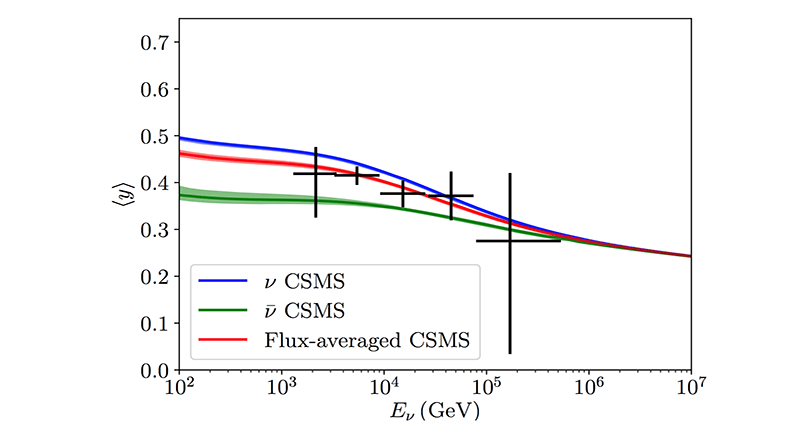
\includegraphics[trim=2.0cm 0.0cm 1.0cm 0.0cm, clip=true, width=\linewidth]{images/inelasticity.png}
    % \end{subfigure}
    \caption{The average inelasticity, $\langle y \rangle$, of neutrino (blue) and antineutrino (green) interactions in IceCube, which differs in the energy range probed in this work~\cite{Aartsen:2018vez}. Reconstructing the inelasticity in IceCube events can thus be used to distinguish (anti)neutrino interactions..}
    % \vspace{-7pt}
    \label{fig:inelasticity}
\end{wrapfigure}

Additionally, within the physics working group I lead the first steps in the detection of delayed light from Michel electrons have been taken, identifying delayed light for $\sim$5\% of events using simple methods and demonstrating the feasibility of this technique. This performance will significantly improve with more sophisticated methods and in particular with the deployment of the IceCube Upgrade, with the far higher sensor density better able to identify the small delayed light signals, and the improved muon track reconstruction allowing the precise position of the muon decay and thus the expected location of the delayed light signal (suppressing `false positive' signals from detector noise). Since the observational of delayed light indicates a muon was present in the interaction products, I will also use this information to improve the existing neutrino flavour classifier that is one of the most important inputs to my current oscillation analyses. 

\begin{wrapfigure}{r}{0.45\textwidth} %this figure will be at the right
    \centering
    % \vspace{-7pt}
    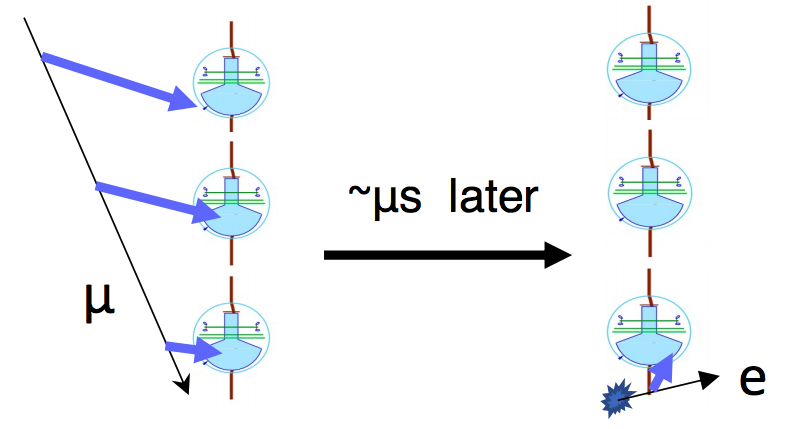
\includegraphics[trim=0.0cm 0.0cm 0.0cm 0.0cm, clip=true, width=\linewidth]{images/michel_electron.png}
    % \end{subfigure}
    \caption{A muon ($\mu$) from a neutrino interaction deposits light in the detector (leading to a reconstructable track) before stopping. Microseconds later the stopped muon decays, producing a Michel electron ($e$) which itself produces detectable light in the nearest sensor. }
    % \vspace{-7pt}
    \label{fig:michel_electron}
\end{wrapfigure}

I will build on these initial studies to pioneer the first use (anti)neutrino separation in IceCube neutrino oscillation measurements. This will require development of inelasticity reconstruction across the full energy-range of IceCube, verification of the theoretical modelling of inelasticity in neutrino event generators and modelling of the associated systematic uncertainty, and development of delayed light tagging methods for the IceCube Upgrade. I will exploit the vast flux of muons from cosmic ray air showers observed by IceCube to develop and verify the delayed light tagging method with high statistics and independently of the neutrino signals, exploiting a synergy with the Niels Bohr Institute (NBI) group of Associate Professor D. Jason Koskinen who are developing a sample of stopped muons in the detector for calibration studies that can also be used and developed in this study. 

I will combine these various methods with correlating data features (such as the reconstructed neutrino energy and direction, and associated uncertainties) to produce a machine learning based (anti)neutrino classifier (for example based on \textit{extreme gradient boosted decision tree ensembles} (REFs, XGBoost, etc) which I have previously used successfully for neutrino flavour classification), assigning each event a probability of being a (anti)neutrino to enable statistical separation of the two cases. Here I will collaborate with my CERN Large Hadron Collider (LHC) colleagues at the NBI (Associate Professor Troels Petersen's group) with whom I am currently undertaking a number of promising machine learning developments in IceCube.

\textbf{Risk:} This a central and highly challenging element of this project, requiring the development and integration of multiple brand new experimental methods. However, a successful (anti)neutrino classifier will be game-changing for IceCube oscillation physics, paving the way for new physics searches with differing (anti)neutrino signals including Non-Standard Interactions (likely yielding the first constraints on the imaginary components of such effects for some couplings), sterile neutrinos and the determining of the neutrino mass ordering, not to mention the $CPT$-V searches in this project. 

I will publish a dedicated paper on these pioneering methods in a suitable technical journal, e.g. the \textit{Journal of Instrumentation}. \\

% A natural future extension of these methods would be to also search for delayed light from neutron capture~\cite{Li:2016kra}, potentially giving the ability to distinguish electromagnetic/hadronic showers in the detector, allowing discrimination of electron and tau neutrino interactions, or neutral currents.

\todo{Antineutrino astronomy}


% TODO important

% \textbf{Pioneer methods to distinguish neutrinos vs antineutrinos}, required by the $CPT$-V measurements. These cannot currently be separated in IceCube oscillation measurements, however properties of the interactions (energy transfer, delayed light from decaying secondaries) can in principal distinguish them. I have recently demonstrated that the energy transfer can be reconstructed in the target energy range in IceCube, and am collaborating with Large Hadron Collider (CERN) colleagues at the Niels Bohr Institute (Associate Professor Troels Petersen's group) to apply state-of-the-art machine learning techniques to tackle this challenge.
% \vspace{2mm} 



\subsection{Detector simulation}

The fundamental method used in these measurements is the comparison of simulated new physics signals and resulting detector response to observed data, and thus a high fidelity simulation model of the new IceCube Upgrade detector is required. I will develop detailed software models of the geometry, active photo-multiplication stage (including spurious pre/after-pulsing) and readout electronics for the new sensors, for the first time utilising the powerful \texttt{GEANT4}(REF) software package (the current `industry standard') for these models within IceCube simulations, replacing the simple and imprecise parametrisations used in existing IceCube simulations. A particular challenge will be modelling the correlated noise across the segmented sensors resulting from the decays of trace radioactive impurities in the glass pressure spheres surrounding the sensors, and calibrating this for every individual sensor. 

% \begin{wrapfigure}{r}{0.4\textwidth} %this figure will be at the right
\begin{wrapfigure}{c}{0.45\textwidth} %this figure will be at the right
    \centering
    % \vspace{-7pt}
    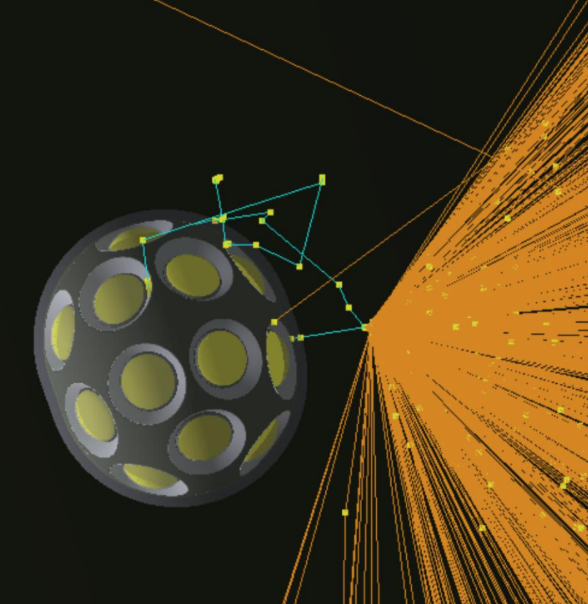
\includegraphics[trim=0.0cm 0.0cm 0.cm 1.0cm, clip=true, width=\linewidth]{images/mDOM_noise.png}
    % \end{subfigure}
    \caption{Visualisation of a prototype GEANT4 simulation of one of the new optical sensors in the IceCube Upgrade. A radioactive decay event is shown.}
    % \vspace{-7pt}
    \label{fig:mDOM_sim}
\end{wrapfigure}

Under my leadership as \textit{IceCube Upgrade simulation manager}, my collaborators and I have taken the first steps in developing simple prototypes of these simulations (see Fig. \ref{fig:mDOM_sim}), which were fundamental to demonstrating the physics potential of the IceCube Upgrade and the successful funding of the project. This, combined with my experience in high fidelity sensor modelling from my Ph.D. (where I developed simulations of the tracking tracking detector the Fermilab muon g-2 experiment, which were a fundamental component of the most precise high energy particle physics measurement in history (REF)) and four years of experience as a professional simulations engineer in the space industry before my academic career (developing simulations of the European Space Agency's ExoMars Rover, Solar Orbiter and GAIA missions), makes me ideally suited to this task. 

A major component of this work will involve verifying and tuning these models against laboratory test data to be taken concurrently by my collaborators in Germany and the US, coordinated via my management role, and finally against the first data from the deployed detector during an initial commissioning phase before physics data runs begin. My team will travel to the South Pole to assist the detector installation, and utilise these simulations to verify the operation of the deployed hardware in real-time. It is therefore crucial that these simulations are complete at the time the detector installation commences, and so this work is prioritised at the start of the project, and indeed this project is critical to the success of the IceCube Upgrade physics program and will be used in all future measurements by this 300-person international collaboration.  

I will publish a methods paper describing these models and the methods employed in a suitable technical journal (e.g. the \textit{Journal of Instrumentation}). \\

% \noindent \textbf{[Task 2]} Produce \textbf{high fidelity simulations of these neutrino interactions and the detector response}, required to test the new physics signals against the observed data and quantify sources of systematic uncertainty. This requires modeling of the new IceCube Upgrade sensors (tuned to calibration data), and state-of-the-art neutrino interaction modelling software will be exploited to accurately simulate neutrino interactions across this vast energy range. \\

\subsection{Monte Carlo Simulation production}

Armed with the new detector simulation models, I will produce high statistics Monte Carlo (MC) simulation samples of both neutrino interactions and background events (atmospheric muons and coincident detector noise) in the detector for comparison to observed data in these measurements. This unglamorous but essential work will require the use of recent developments in the state-of-the-art neutrino event generator software \texttt{GENIE} (REF) to for the first time accurately and consistently model neutrino interactions across the many orders of magnitude in neutrino energy probed in this project, particularly in the 100-1000 TeV region which marks the transition between two distinct neutrino cross section calculations. Additionally, I will integrate cross section tuning data provided by accelerator neutrino experiments based on their dedicated neutrino cross section measurements. This work will benefit from my extensive experience with large scale distributed grid computing, which I have successfully employed in the current generation of IceCube oscillation analyses.

\textbf{Risk:} Simulating the extremely high rates of background events observed in the IceCube Upgrade is computationally challenging, potentially creating a bottleneck in these measurements. The simplest mitigation strategies in such a situation is implementing hard cuts in the data sample to sharply suppress backgrounds, at the cost of loss of neutrino events and thus measurements sensitivity. I will also investigate (potentially as MSc projects) new methods for faster background simulation, including parameterising computationally expensive aspects of the simulation, or exploiting cutting edge \textit{generative} machine learning methods to `learn' the event distributions. Both of these methods could significantly reduce the computational load of background MC production, and have been successfully employed at the LHC in recent years (REFS). \\


\subsection{Event sample}

At the core of these measurements will be the first \textbf{atmospheric neutrino data sample spanning the full energy reach of IceCube} (GeV to PeV), containing over \textbf{1 million neutrinos} to provide unprecedented statistics for neutrino physics. This is necessitated by the broad energy range of potential signals probed in this project, and to maximise the sensitivity to the suppressed signals of quantum gravity at even the highest energies I will probe. Both data from the IceCube Upgrade and existing IceCube data (totalling more than 10 years of livetime) will be used to maximise the statistics. The core challenges of the event sample are the rejection of the overwhelming atmospheric muon and coincident noise backgrounds that dominate the detector data (thousands or even millions of which are observed for every neutrino) to yield a pure sample of neutrino events, and to reconstruct the properties of these neutrino interactions (for example the energy, direction and flavour of the incoming neutrino and the resulting interaction products).

To create this holistic neutrino sample I will unify the disparate existing methods developed by myself (GeV energies) and my collaborators (TeV energies) -- each developed for particular neutrino energy range and event topology (for example fully vs. partially contained events, track-like events from muon neutrino interactions vs. spherical light emission from electron/tau neutrinos, etc) -- and develop them further to integrate the data from the new IceCube Upgrade sensors into these methods. The high noise rates in these new sensors result in coincident noise background rates orders of magnitude higher than for the existing IceCube detector, and isolating and removing these events will be critical to this project. I developed the current leading methods for noise rejection in IceCube (being the first to exploit machine learning), which remove events with light emission that is not causally consistent with a common origin, and will significantly expand these methods exploiting the segmented nature and dense spacing of the new sensors\todo{More specific details would be nice here}.

\textbf{Risk:} The existing methods used for reconstructing neutrino properties in IceCube do not naturally extend to supporting the new IceCube Upgrade sensors or the irregular detector geometry, meaning new techniques must be developed. The development of deep learning neural network based reconstruction methods that are not tied to the regular pixel structure of standard image processing techniques (which dominate much of the machine learning community) is well underway within the IceCube collaboration however, including a graph neutral network (GNN) based method resulting from my aforementioned collaboration with NBI machine learning experts from the ATLAS experiment, which has already demonstrated $\sim$30\% improvement in resolution over the current state-of-the-art methods in IceCube. However, should these methods not achieve maturity in time for these measurements, I can fallback to existing non-machine learning reconstruction methods with relatively simple modifications, but at the cost of failing to exploit the segmented nature of the sensors (resulting in degraded performance and thus a loss of measurement sensitivity). \\

%All previous IceCube analyses have probed only subsets of IceCube's data, reducing the sensitivity and robustness of results (for example by eliminating off signal control regions) and potentially contributing to inconsistencies between existing IceCube results and providing `gaps' in parameter space where signals can be missed\todo{Turn this sentence into a risk/gain?}. 



\subsection{Atmospheric muon sideband}

Although the new calibration devices in the IceCube Upgrade will greatly reduce the impact of systematic uncertainties related to the properties of the detector and in particular the optical properties of the ice, the composition of the atmospheric neutrino flux remains a major source of systematic uncertainty due to uncertainties in the spectrum of cosmic rays reaching the Earth, atmospheric conditions, and the modelling of hadronic processes governing the air shower development. However, in addition to neutrinos these air showers also produce a copious flux of muons, $\mathcal{O}(10^5)$ of which are detected in IceCube for every neutrino observed. 

I will develop a high statistics data sample of well reconstructed muons in IceCube and simultaneously fit this data sideband alongside the neutrino data during these measurements, strongly constraining the air shower uncertainties independently of the neutrino physics signals and increasing both the sensitivity and robustness of these measurements. This will be the first use of this novel method in IceCube, and will be invaluable in giving confidence in any detected new physics signal. \\

\todo{`control sample'}


% - Sys dominated
% - Flux + detector sys
% - Calibration only for detectopr sys, plus only helps some strings
% - Synergy with verifying delayed light

\subsection{Systematic uncertainty modelling}

% - New detector modules and hole ice
% - New calobration
%  - Dedicated noise component sys uncertainties
% - Sim studies, using experience from this prpject (sim + OM testing)

The high precision of the measurements proposed here (afforded by the high statistics data sample) and the potentially small signals being sought necessitate a robust treatment of systematic uncertainties. Uncertainties related to the detector will include the calibration of the quantum efficiency, noise rates and position/orientation of the new optical sensors -- which are deployed down 2 km long cables into melted and subsequently re-frozen boreholes in the ice -- and the optical properties of these re-frozen ice columns. I will perform dedicated simulation studies of these effects and derive analytic parameterisations of the resulting impacts on the reconstructed properties of the neutrinos for use in the $CPT$-V and decoherence measurements (where the uncertainties are represented as \textit{nuisance parameters} in the fit). The expertise my group will have developed in detector simulation and with the data from laboratory testing of the sensors will be invaluable to this work.

I will also integrate relevant advances from my collaborators into the measurements, including improved constrains on the bulk optical properties of glacial ice in which IceCube resides (achieved using new clibration devices deployed with the IceCube Upgrade), and advances in atmospheric neutrino flux modelling currently under development by a student at NBI. \\

\todo{Risk of discover of new systemtics that are time consuming to deal with}

\subsection{Signal modelling}

These measurements will test the influence of quantum gravity on neutrino propagation in a number of models, many for the first time, and these effects must be precisely calculated when computing the simulated signals of these effects in the detector. I will implement these models using the state-of-the-art \texttt{nuSQuIDS} quantum state evolution software~\cite{Delgado:2014kpa, nusquidsGIT}, and integrate them to my sophisticated neutrino data analysis framework. In particular, this will allow accurate modelling of the interplay between new physics effects and the influence of standard matter in the Earth on neutrino propagation (including absorption of high energy neutrinos by the Earth), which has been neglected in many earlier decoherence studies (in some cases leading to spurious signal artefacts)~\cite{PhysRevD.97.115017}. I have experience in this area having already implemented my $\nu$-VBH interaction model using \texttt{nuSQuIDS}, and was the first to properly integrate Earth matter effects in the modelling of decoherence in atmospheric neutrinos.

Both decoherence and $CPT$-V have been predicted from varied new physics scenarios, meaning these measurements are potentially sensitive to the properties of \textit{strings/brane} theories (so-called \textit{grand unified theories})~\cite{Mavromatos2010, AmelinoCamelia:2008qg}, new fermionic particles~\cite{Hellmann:2021jyz}, neutrino interactions with Dark Matter~\cite{1909.11271, EPJC802020} and a diffuse gravitational wave background~\cite{PhysRevD.100.096014}.  To this end I will host a specialised workshop on neutrino decoherence and $CPT$-V to further develop these scenarios (drawing upon the \textit{COST Action CA18108 (quantum gravity phenomenology)} network of which I am an active member) with a view to testing further models in this project, and expect to create a number of MSc projects developing this phenomenology (potentially yielding dedicated publications).

I will release all models developed in this work as open source software, allowing other experimental collaborations to test these signals.  \\

\subsection{$CPT$-V analysis}

The event sample and simulations developed in this project will form the core of both the $CPT$-V and decoherence analyses, both of which will also utilise my existing oscillation analysis framework, modified to include the new systematic uncertainty and signal modelling. The measurements will search for distortions in the atmospheric neutrino spectrum in IceCube in 4-dimensions; reconstructed neutrino energy, arrival direction (a proxy for travel distance), particle type (using the topology of the event to distinguish between muon neutrino interactions with track-like topologies vs all other cases, which are roughly spherical in nature), and neutrino vs antineutrino (using the new methods developed in this project).

For the $CPT$-V search I will test the data for the presence of differing oscillation properties between (anti)neutrinos using a phenomenological parameterisation of these effects of my own devising, yielding the world's first energy-dependent search. The parameterisation is of the form $\Delta \theta = \epsilon (E/\Lambda)^n$, where $\Delta \theta$ is the difference in value of a given neutrino oscillation parameter for neutrinos and antineutrinos, $E$ is the neutrino energy and $\Lambda$ is the energy scale of the new physics producing the $CPT$-V effects, and $\epsilon$ and $n$ characterise the scale and energy-dependence of the effects respectively. This form is equivalent to the energy-independent tests performed in previous measurements when $n=0$, allowing easy comparison of my results with previous literature. The parameters $\epsilon$, $\Lambda$ and $n$ will be fit parameters in the analysis, and additionally specific cases can be tested if compelling model predictions are found (for example a prediction of $\Lambda$ for a new physics theory) \todo{Do I actually need to outline this parameterisation?}. I will test the possibilities that both the mixing properties of neutrino mass/flavour states (e.g. the mixing angles, controlling the amplitude of neutrino oscillations) and neutrino masses (e.g. the mass splittings, controlling the oscillation frequency) differ for (anti)neutrinos. 

\textbf{Risk:} The success of this measurement will be strongly affected by the performance of the (anti)neutrino separation methods developed in this work. A delay to the installation of the IceCube Upgrade would also affect this result, but the timeline is such that even a delay or one year would still yield at least one year of physics data for the measurement, which will be supplemented with existing IceCube data \todo{Try to turn these into positive sentences}.

A signal detection in this measurement would be a momentous result, giving one of very few experimental signs of the new physics we know must exist beyond the Standard Model of particle physics and likely motivating a slew of new models from the theoretical community seeking to explain the observation. In such a case I will target the high profile journal \textit{Nature} to publish these results, whilst if no signal is observed I will place the world's first constraints on energy-dependent $CPT$-V effects in neutrinos and target the journal \textit{Physical review Letters}\todo{DO I actually need to discuss papers for ERC?}. \\

\subsection{Decoherence analysis}


\begin{figure}
%\begin{subfigure}[t]{0.5\textwidth}
    \begin{subfigure}[b]{0.5\textwidth}
    \centering
    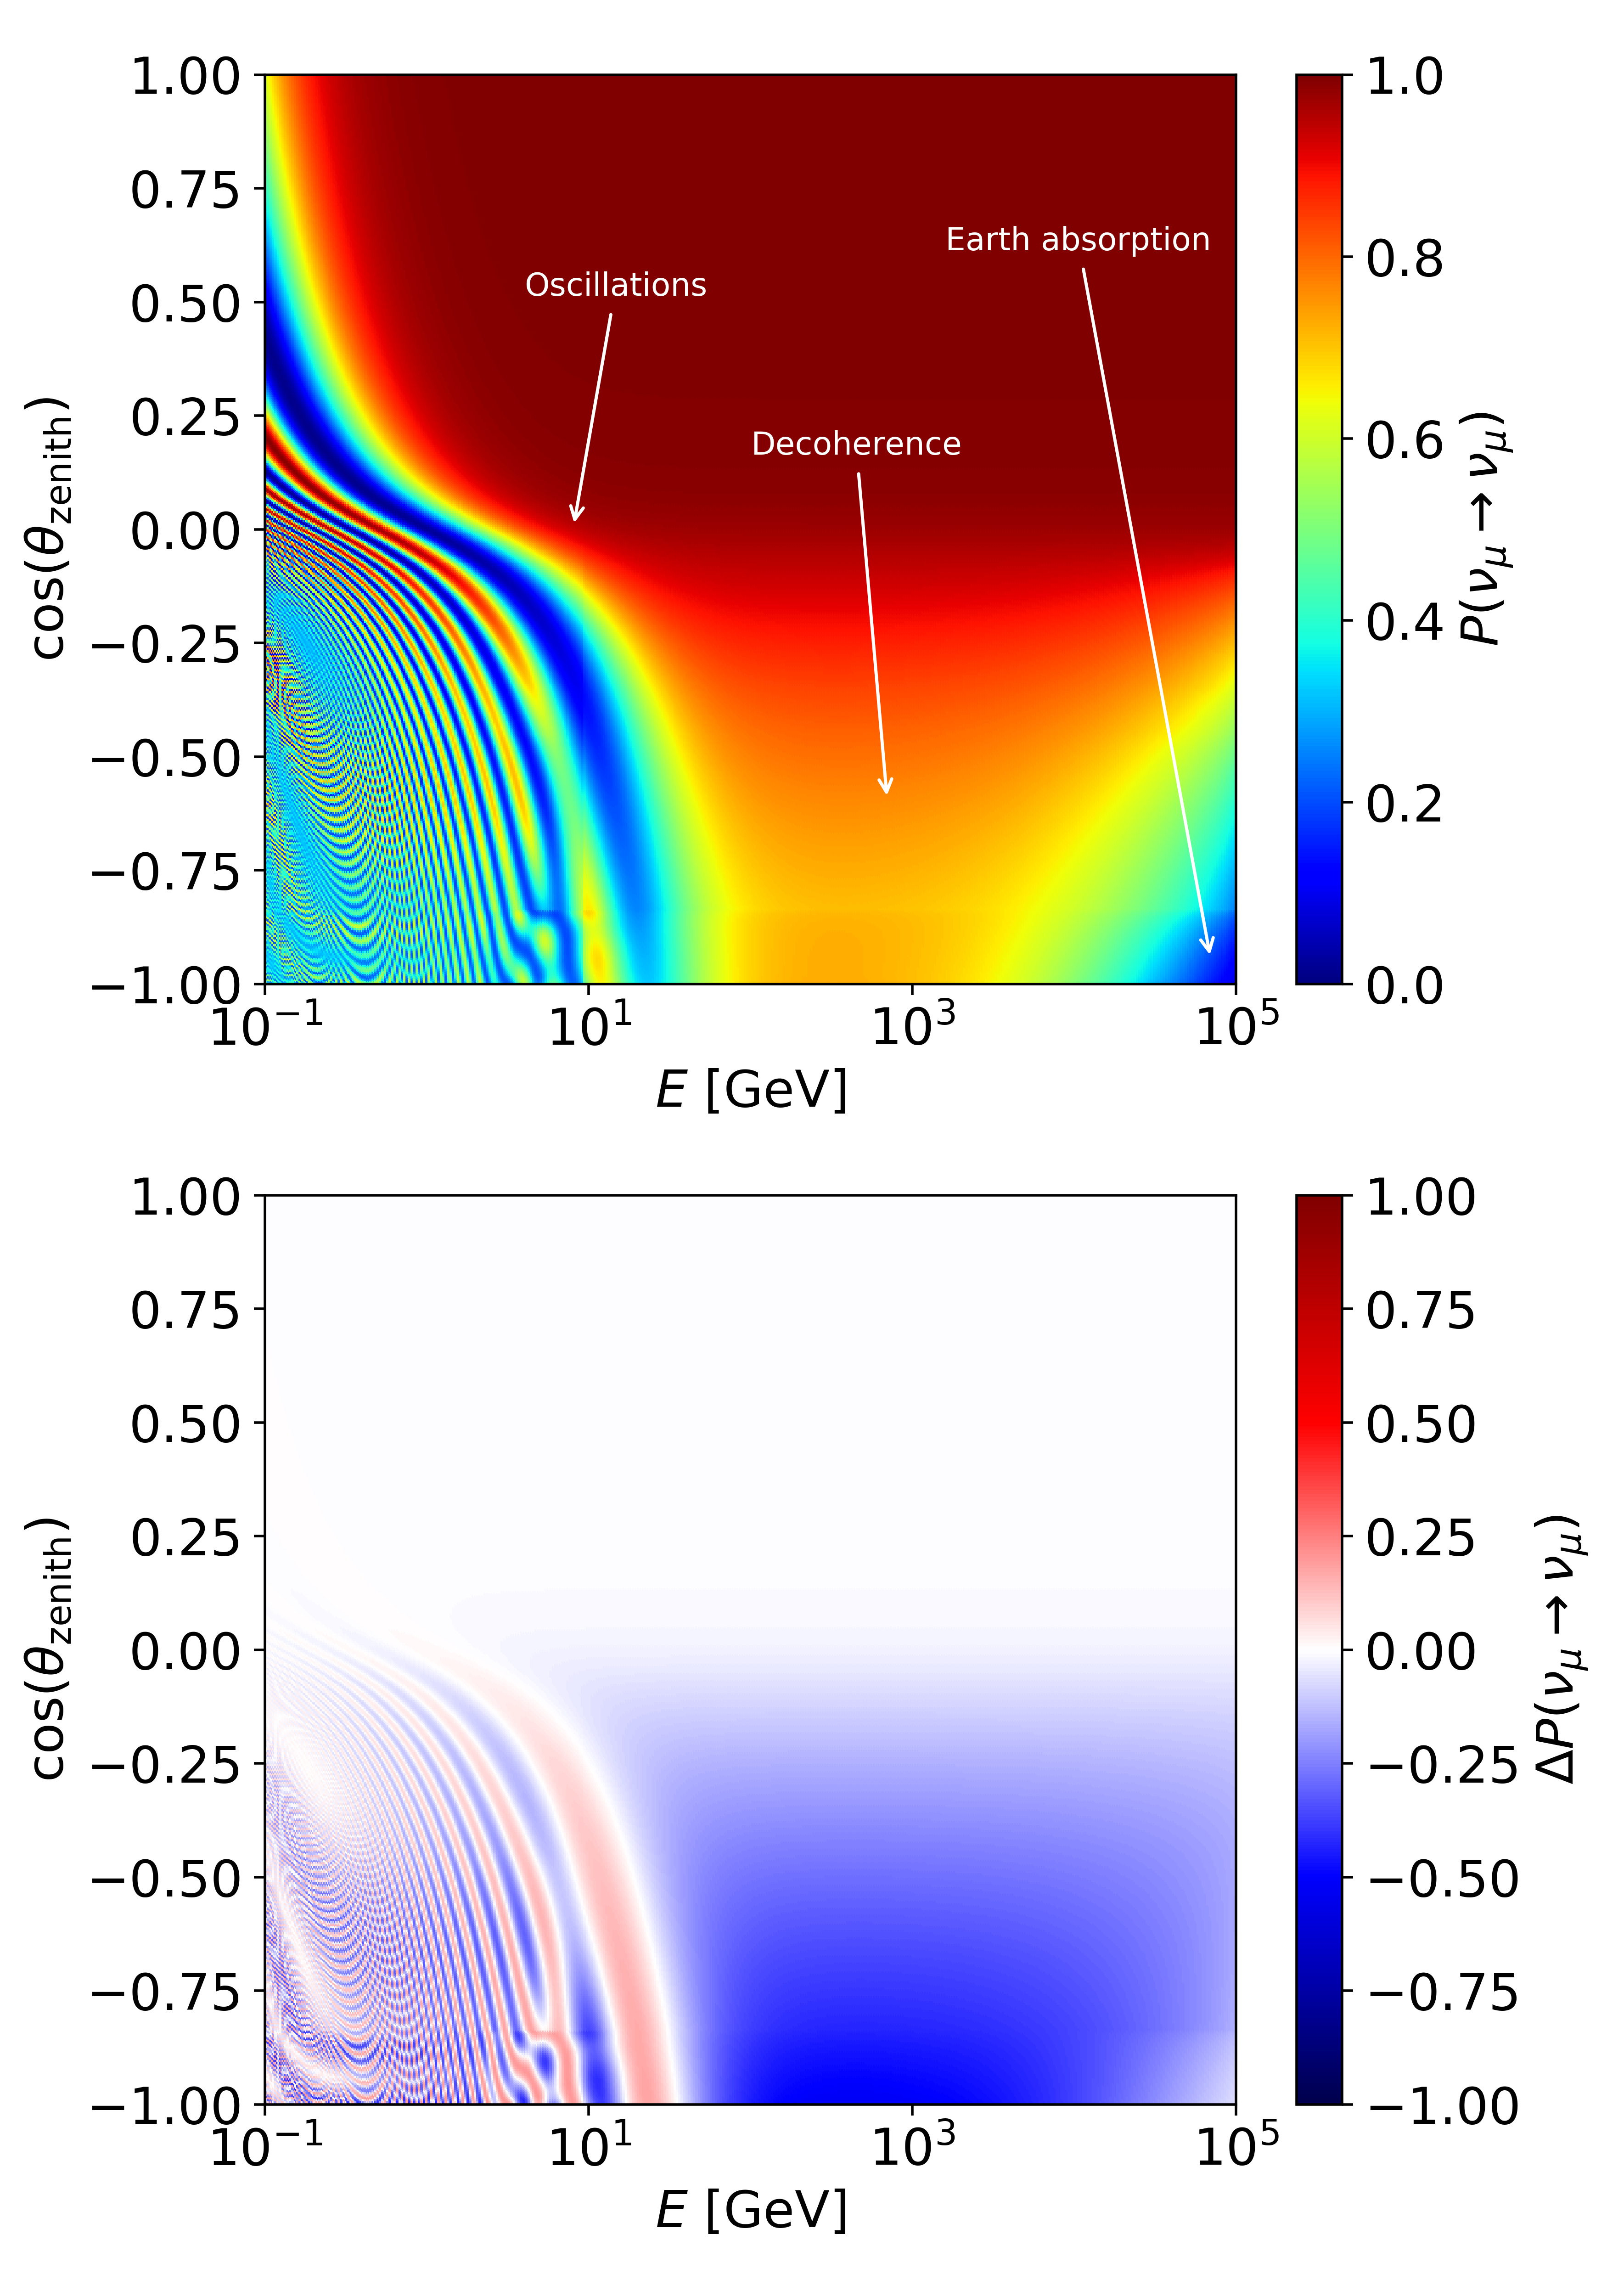
\includegraphics[trim=0.0cm 12.7cm 0.cm 0.2cm, clip=true, width=\linewidth]{images/atmo_oscillogram_randomize_flavor_n0_matter.png}
    \caption{\label{fig:CryoDarkRate}}
    \end{subfigure}
    \begin{subfigure}[b]{0.5\textwidth}
    \centering
    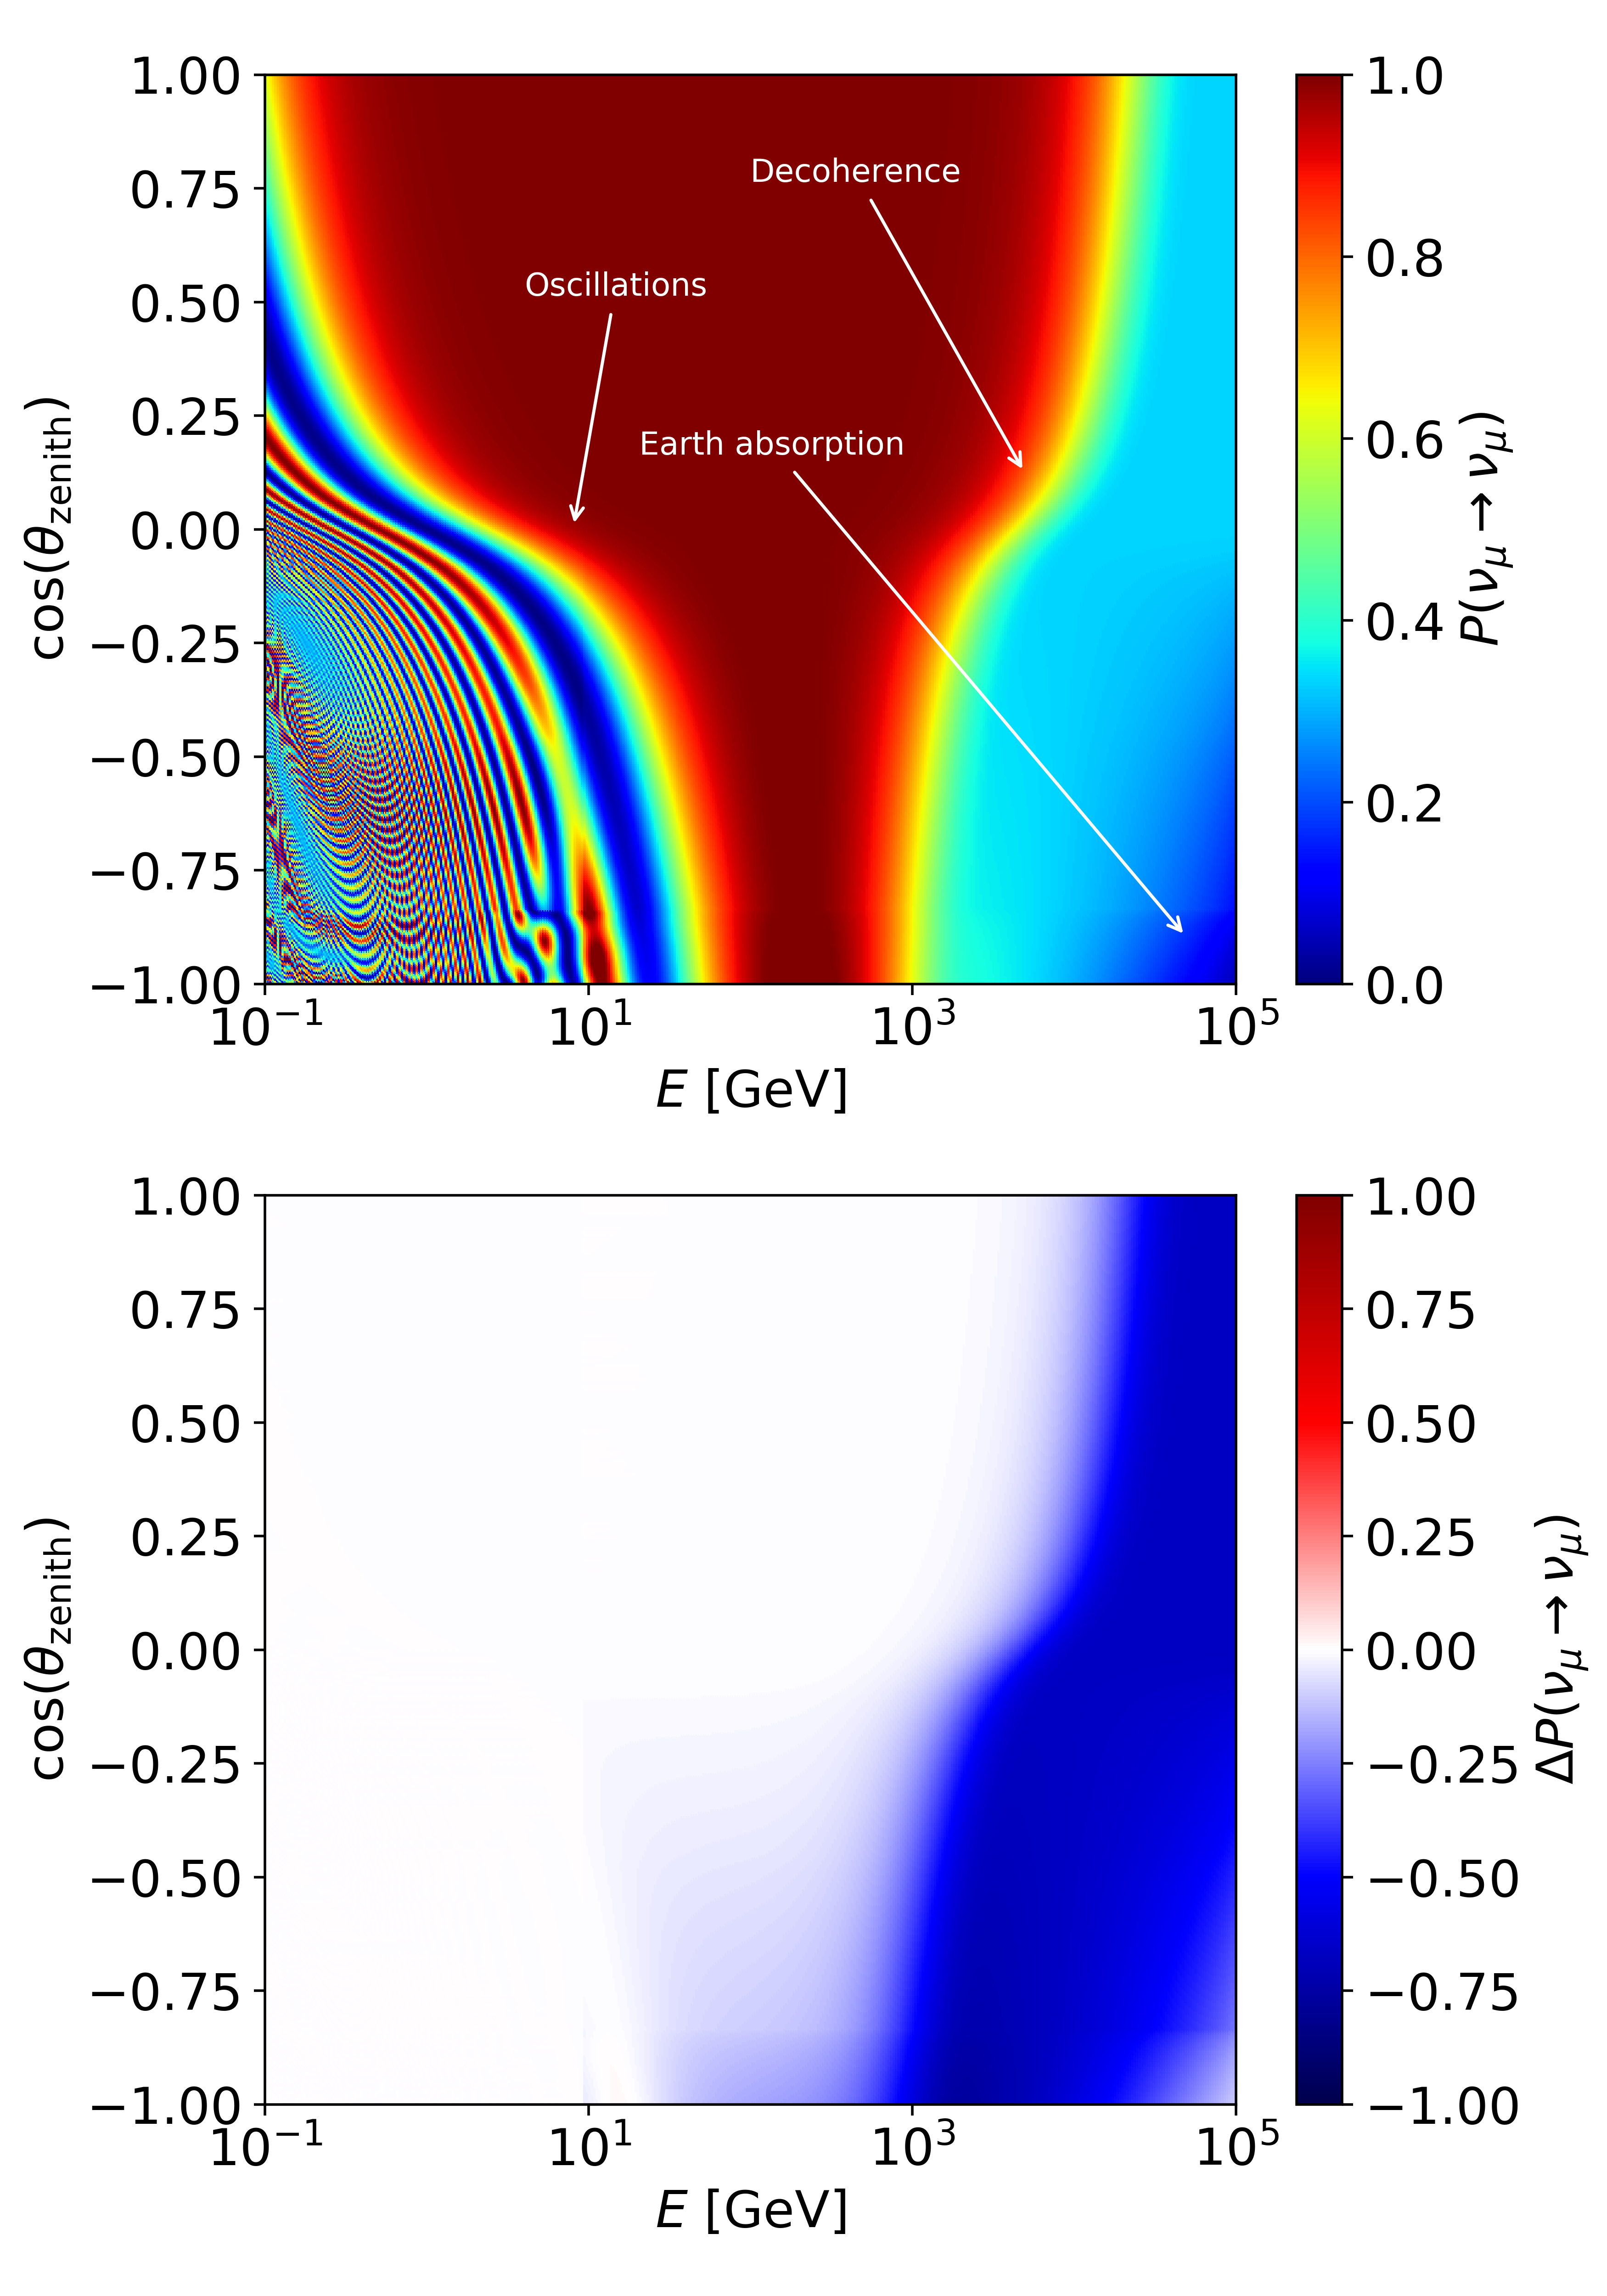
\includegraphics[trim=0.0cm 12.7cm 0.cm 0.2cm, clip=true, width=\linewidth]{images/atmo_oscillogram_randomize_flavor_n2_matter.png}
    \caption{\label{fig:mDOM_noise}}
    \end{subfigure}
    \caption{Modified atmospheric neutrino oscillations vs. neutrino energy (x axis) and arrival direction (y axis) in my $\nu$-VBH interaction decoherence models, showing (a) energy-independent and (b) $E^2$ suppressed scenarios (to which accelerator experiments are blind)~\cite{PhysRevD.102.115003}. Detectable features are present across a broad range of energies.}
    \label{fig:decoh_oscillograms}
\end{figure}

% \begin{wrapfigure}{r}{0.5\textwidth} %this figure will be at the right
%     \centering
%     \vspace{-7pt}
%     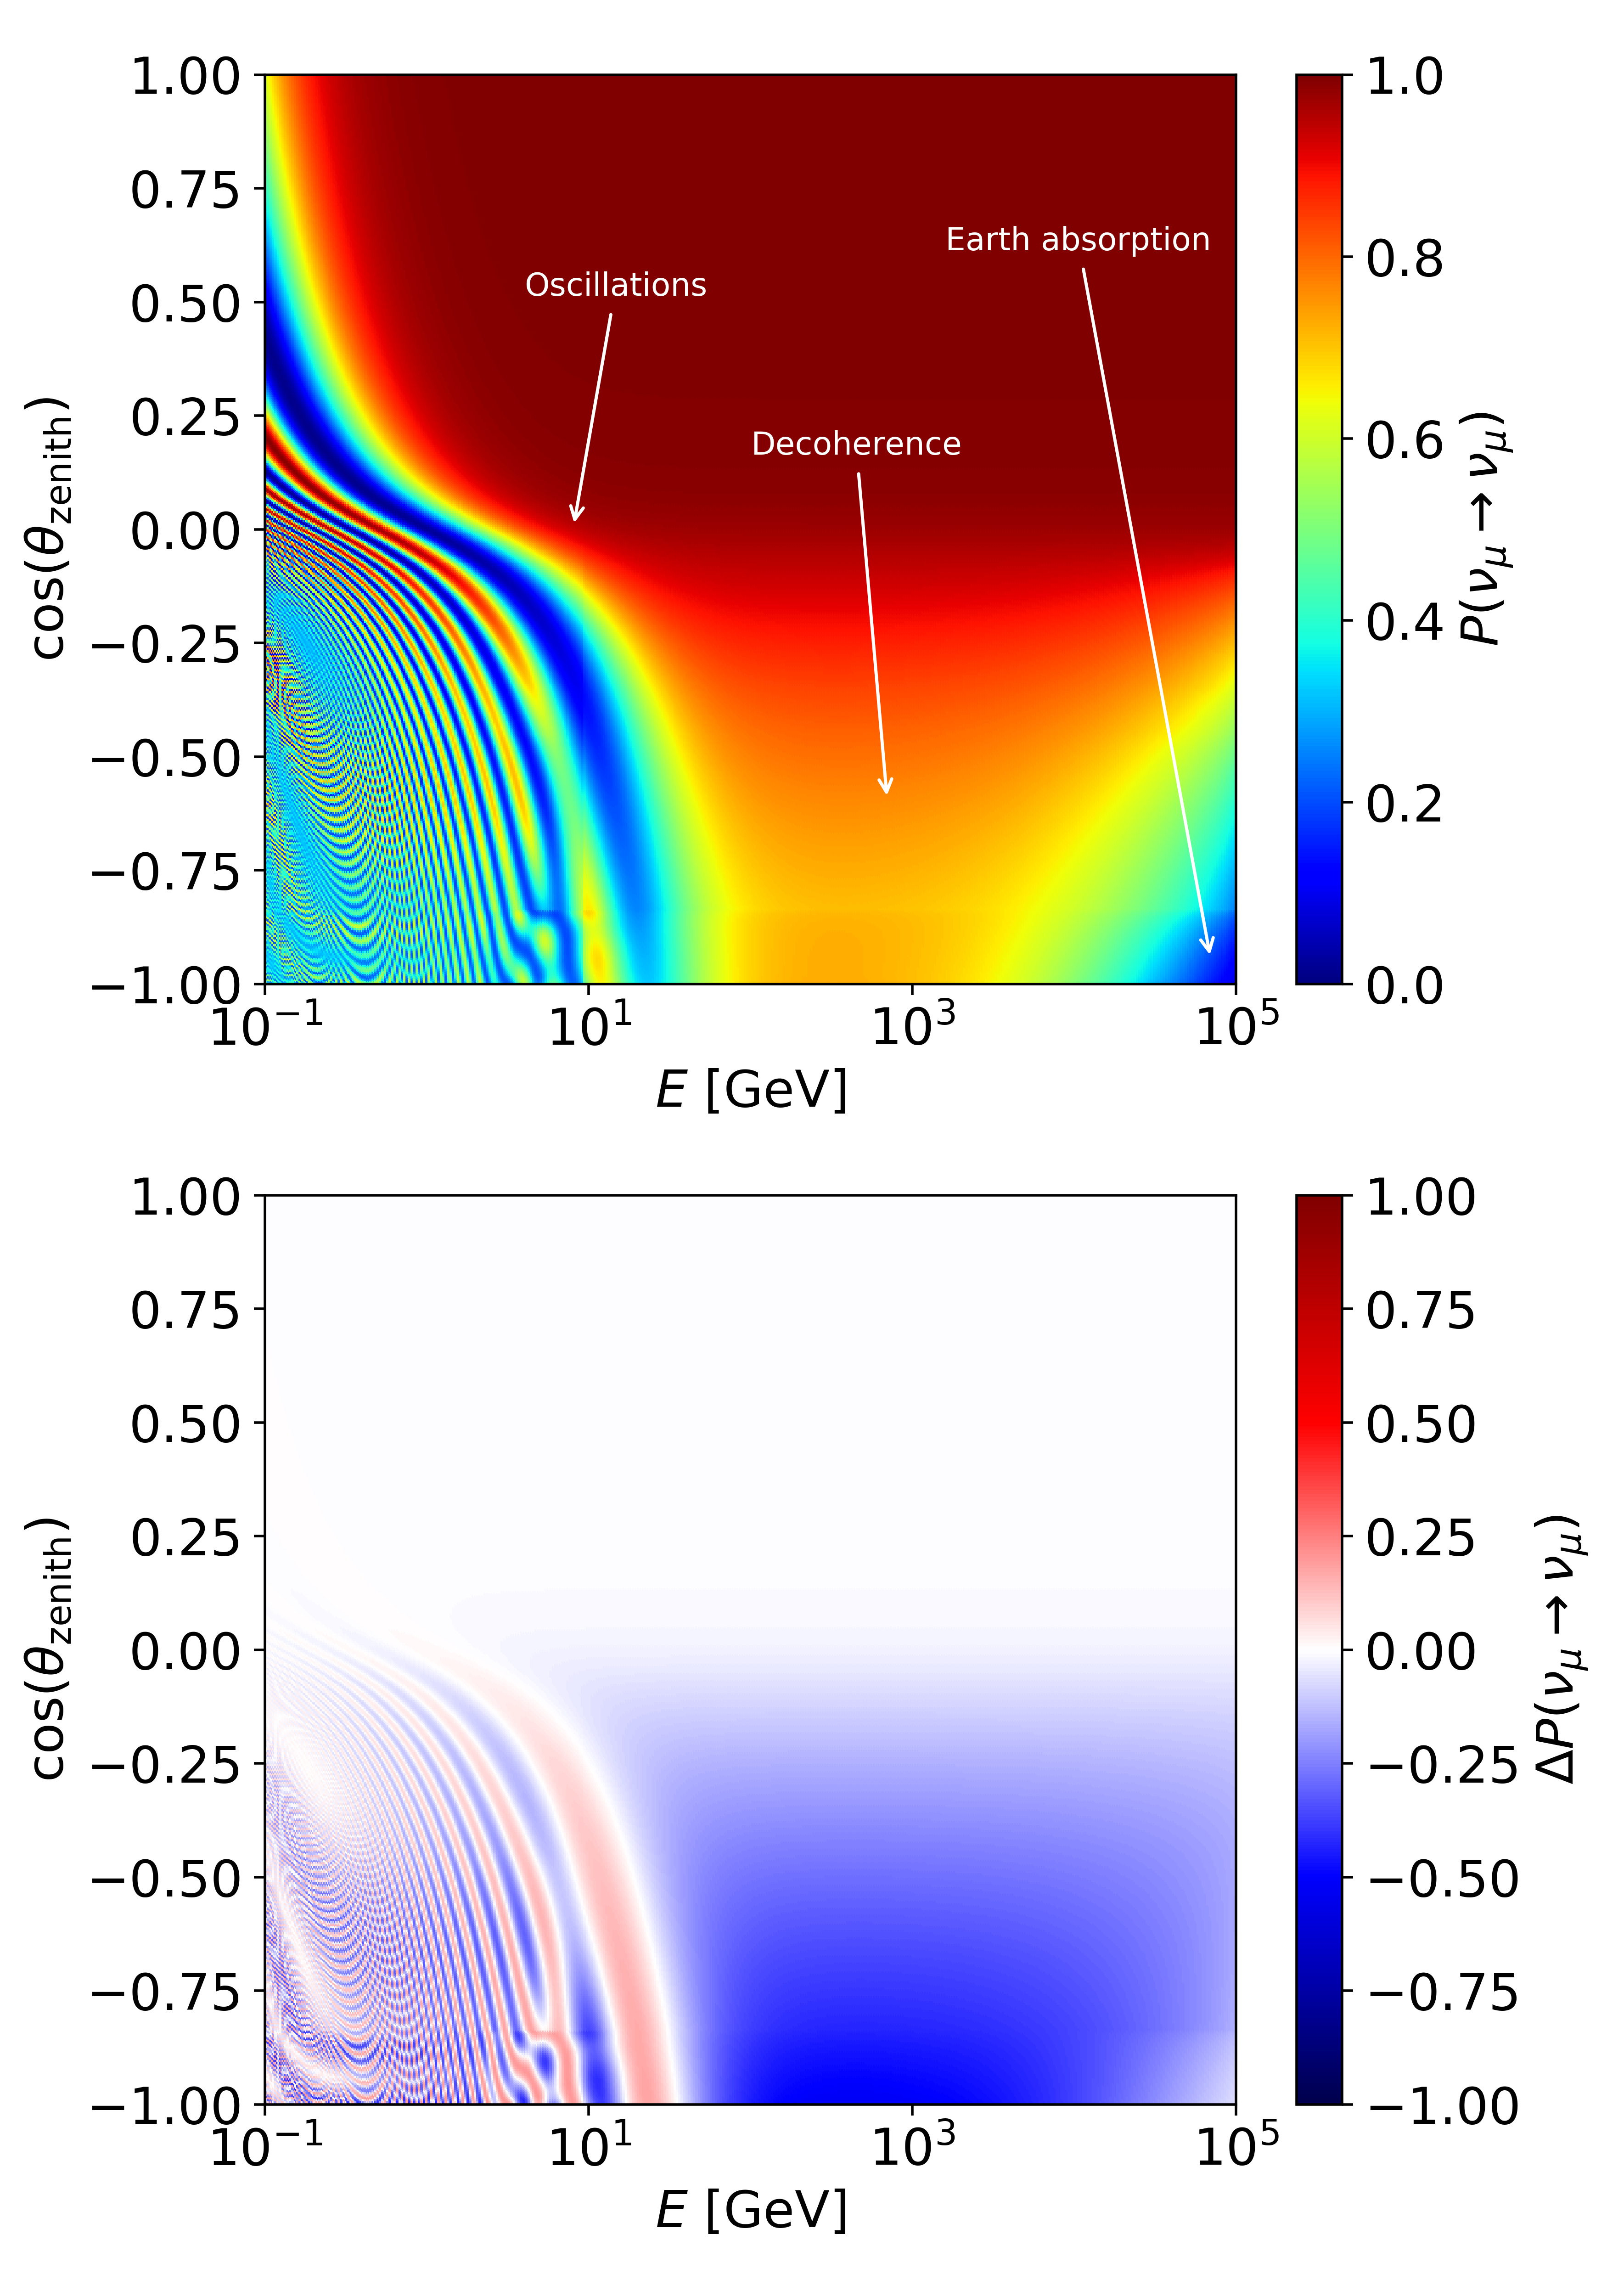
\includegraphics[trim=0.0cm 12.7cm 0.cm 0.2cm, clip=true, width=\linewidth]{images/atmo_oscillogram_randomize_flavor_n0_matter.png}
%     % \end{subfigure}
%     \caption{Modified atmospheric neutrino oscillations (vs neutrino energy and direction) in one of my $\nu$-VBH interaction decoherence models. Detectable features are present across a broad range of energies.}
%     \vspace{-7pt}
%     \label{fig:decoh_oscillograms}
% \end{wrapfigure}
% \todo{E2 fig}

The signal of neutrino decoherence in IceCube is the damping of neutrino oscillations over distance, in particular resulting in the appearance of tau-flavour neutrinos outside of the conventional oscillation signal region, with the signal strongest for neutrinos crossing the full diameter of the Earth before detection. In the absence of a complete theory of quantum gravity I will test a range of energy-dependent scenarios, with signals manifesting across the full energy range of the event sample developed in this project (see Fig. \ref{fig:decoh_oscillograms}).

In this search I will test a range of decoherence models (a number of which I developed), including $\nu$-VBH interactions and lightcone fluctuations, fitting the underlying model parameters. This work will yield the \textbf{first ever measurements}\todo{Not really first due to LBL paper?} of the $\nu$-VBH interaction mean free path (in turn constraining how numerous VBHs are and how strongly they interact with neutrinos), the size of the space-time fluctuations experienced by neutrinos, and the intrinsic variability of neutrino velocity. I will also test the possibility that neutrinos can decay, since it shares common damping features to the decoherence signals I am probing, increasing the physics output of this work.

I will also perform a model-independent decoherence search, fitting the matrix elements of a generalised \textit{decoherence operator} (expressed in the mathematical framework of \textit{open quantum systems} (REFS), the world's first measurement of this kind. This will maximise the sensitivity of the analysis to decoherence from any source, invaluable given the breadth of new physics scenarios potentially producing decoherence effects. 

% \textbf{Risk:} This generalised decoherence search will feature many free parameters in the fit, a major computational challenge for the frequentist \textit{minimisation} algorithms used in most oscillation analyses. Should this prove untenable, I will instead employ Bayesian Markov Chain Monte Carlo (MCMC) methods which have been shown to perform better in many parameter fits. This will require a significant time investment implementing these methods in my analysis software framework\todo{Probably drop this - boring}.

There is also an exciting synergy between the searches proposed in this work. A frequent prediction in quantum gravity phenomenology is that $CPT$-V manifests as differences between neutrino and antineutrino decoherence effects~\cite{Mavromatos_2009, Barenboim:2004wu, Carrasco:2018sca, Buoninfante:2020iyr, Capolupo:2020myw}. This hypothesis has never been experimentally tested, and I will perform the world's first search for $CPT$-V decoherence in this project (having recently demonstrated the feasibility of detecting such signals in IceCube), yielding the prospect of detecting $CPT$-V even if the neutrino-antineutrino oscillation asymmetry effects discussed above prove immeasurably small \todo{Actually an intrinsic connection between $CPT$-V and decoherence}.

\todo{More specific at what models can be rejected, e.g. VBH ones}

This work will be by far the most sensitive and comprehensive search for energy-suppressed neutrino decoherence ever performed. These results will achieve sensitivity to the naturally expected scale of quantum gravity effects for a number of the models tested \todo{More specific?}, giving genuine hope of the first quantum gravity signal detection, a truly revolutionary result. A null result in these models will reject all but the most energy-suppressed Planck scale decoherence scenarios, or indicate that their effects are much weaker than predicted. Either way these results will be invaluable in informing the theoretical development of quantum gravity. For the publication of the results I will target the high impact journal \textit{Nature} since it is guaranteed to either detect or rule out the natural Planck scale expectation for some models. I also may split the multiple scenarios tested into separate publications. \\

% The impact of a signal detection would be revolutionary, giving one of very few experimental signatures currently known of physics beyond the Standard Model. Follow-up would include testing these signals in other experiments (such as next-generation atmospheric neutrino experiments such as ORCA, HyperKamiokande and the Indian Neutrino Observatory, or the DUNE accelerator experiment), or indeed in non-neutrino experiments, and would likely result in a slew of new theoretical models to be compared to the experimental data. \\

\todo{Proton decay}
\todo{E3}


\subsection{Project management}

\begin{figure}[h]
	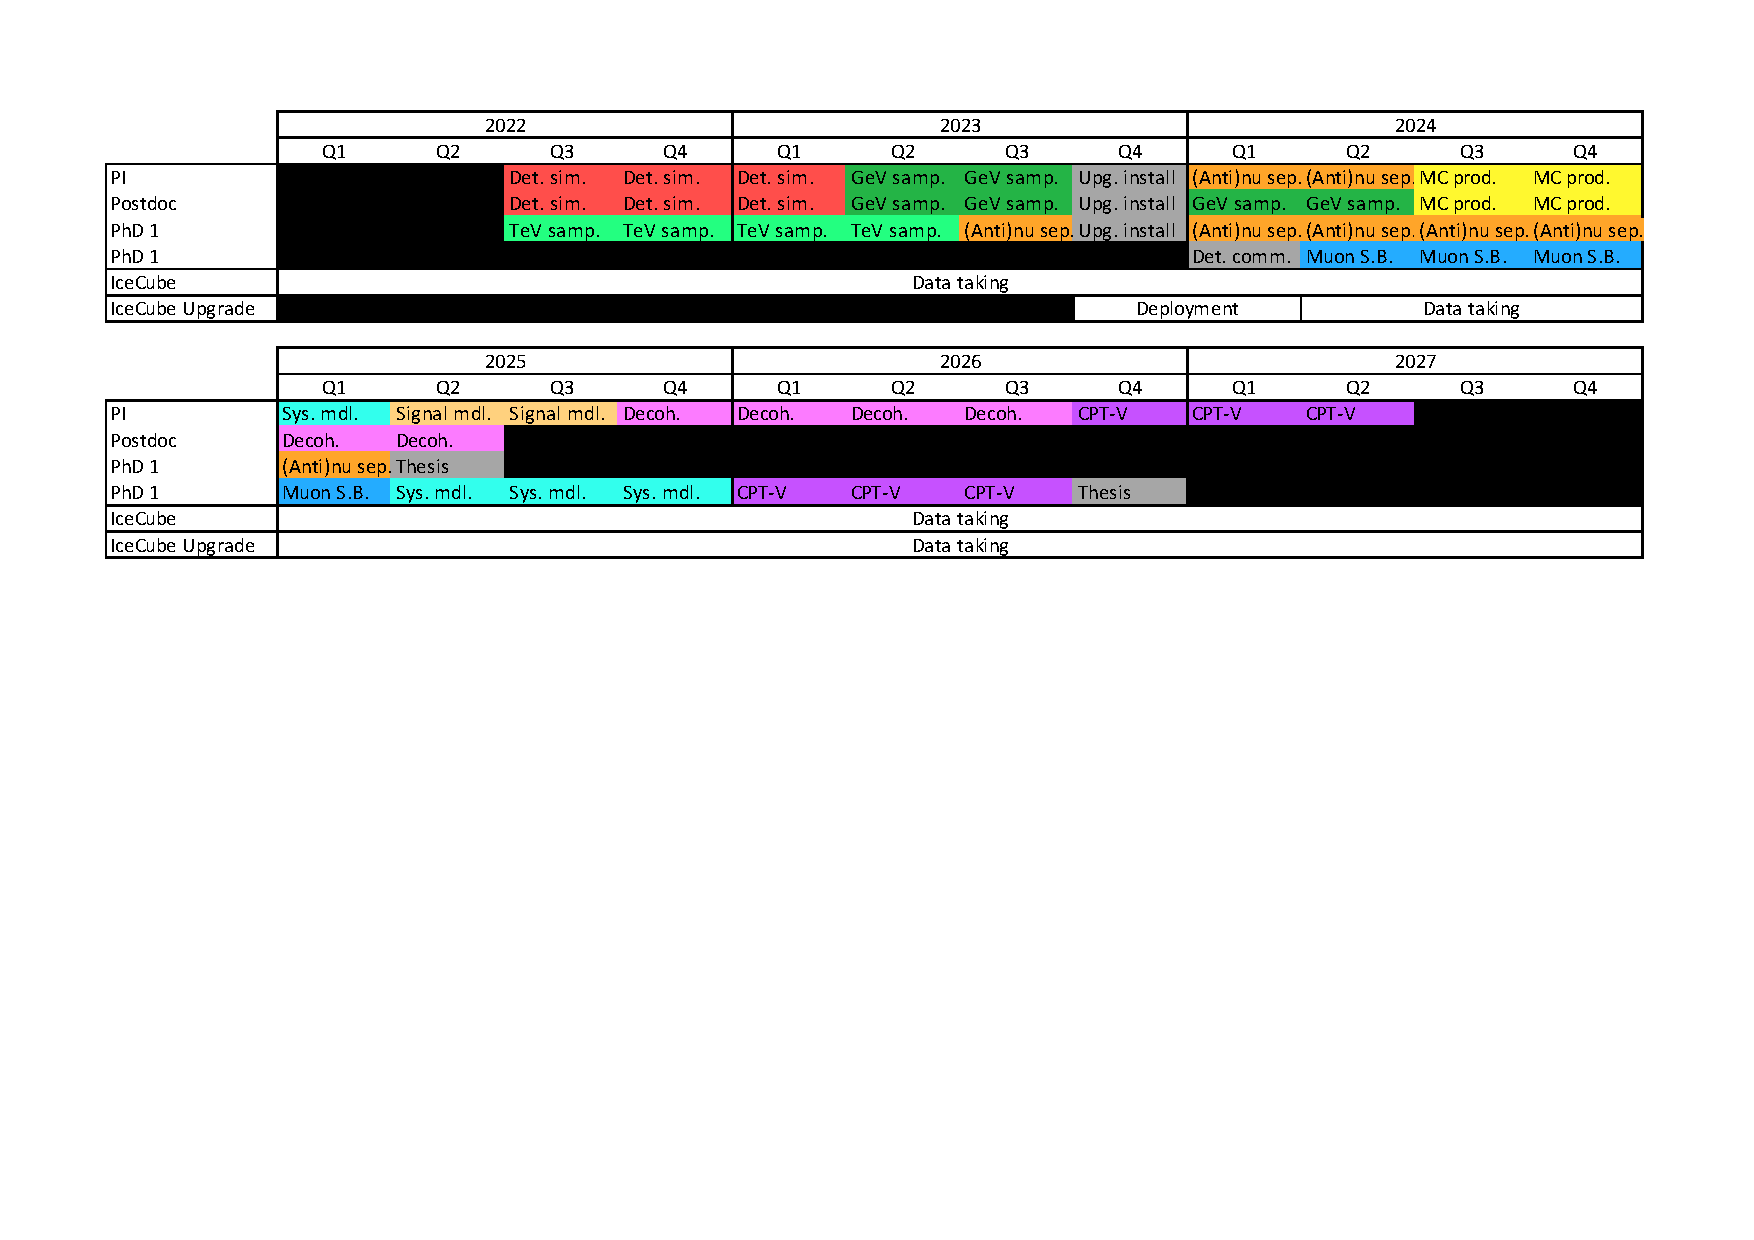
\includegraphics[trim=1.7cm 11.1cm 1.7cm 1.0cm, clip=true, width=0.99\linewidth]{images/TaskPlanning.pdf}
	\caption{Project timeline for all team members and the IceCube (Upgrade) detector.}
% 	\vspace{-12pt}
	\label{fig:timeline}
\end{figure}


\begin{wrapfigure}{r}{0.5\textwidth} %this figure will be at the right
    \centering
    % \vspace{-7pt}
    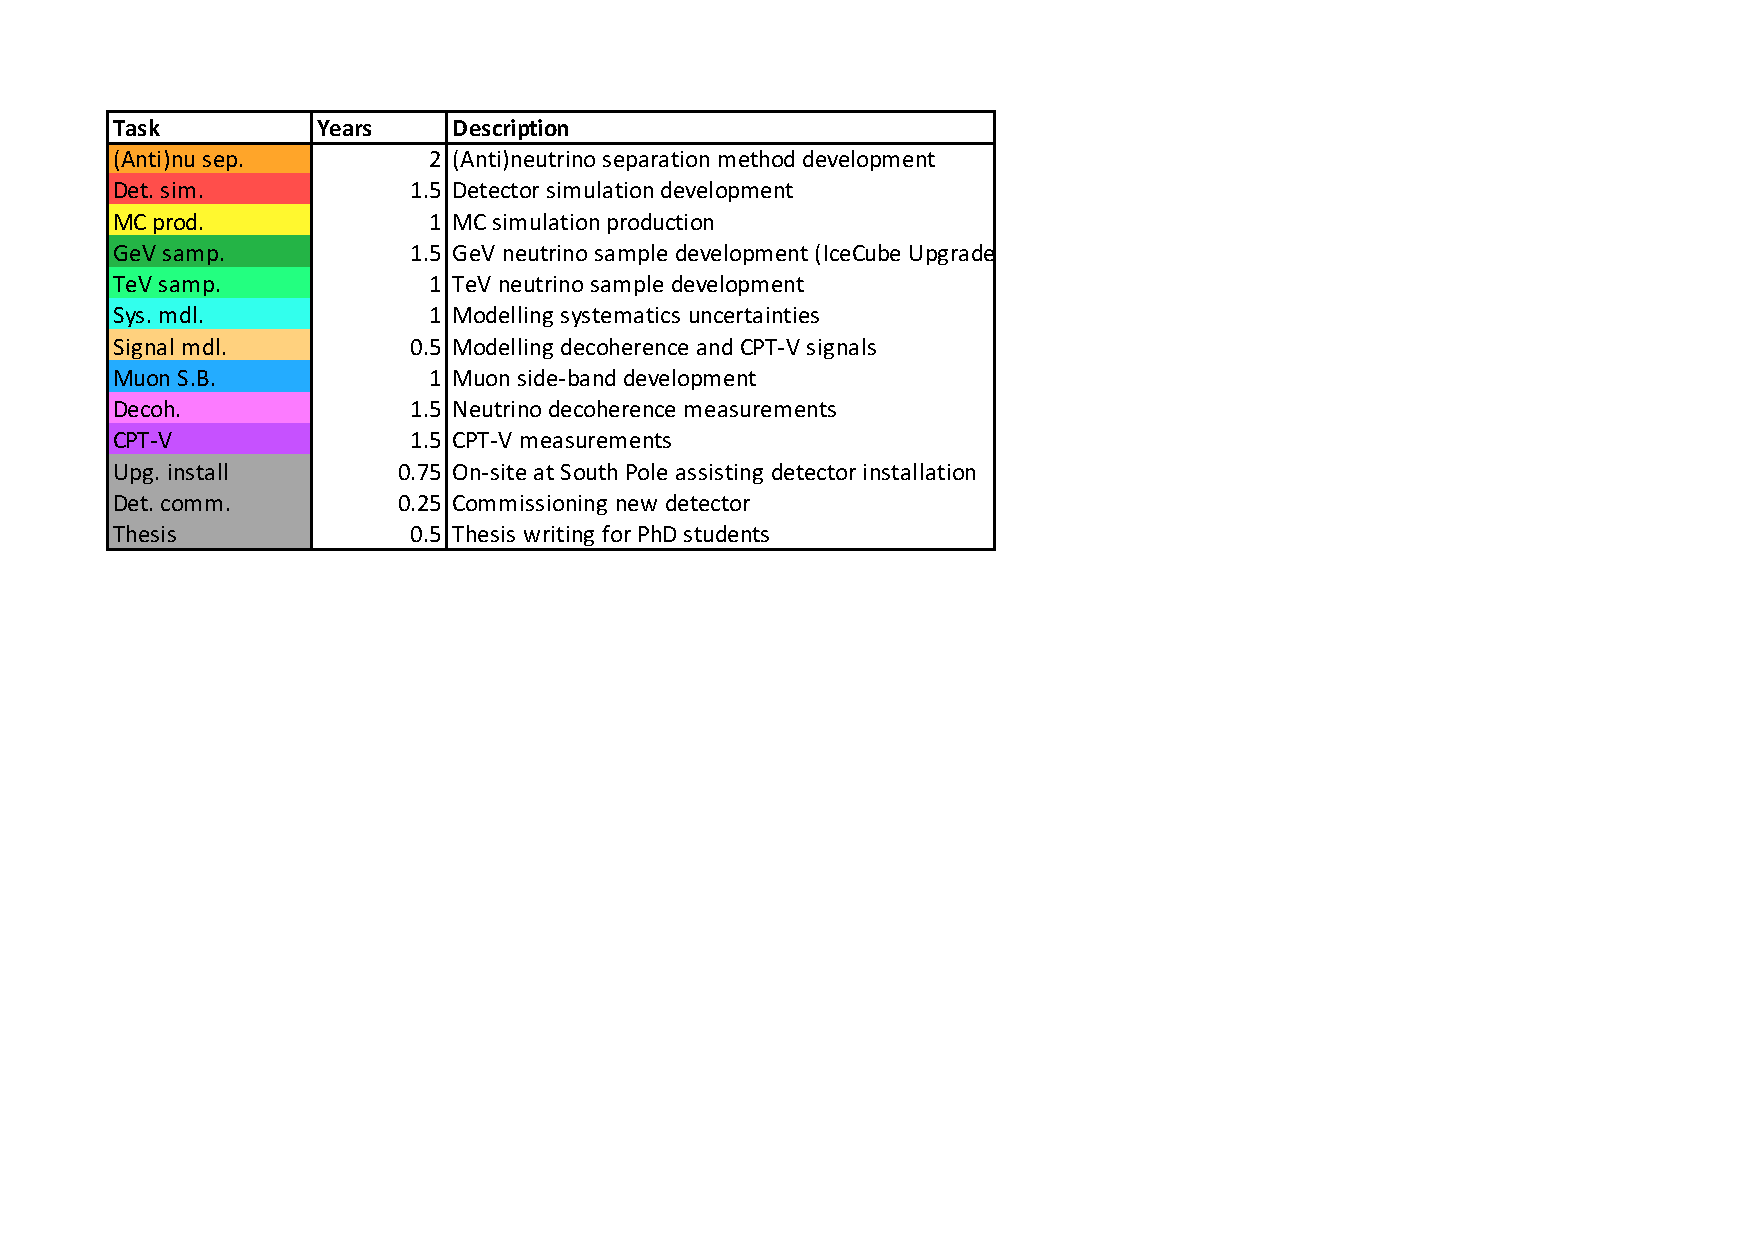
\includegraphics[trim=1.7cm 11.5cm 12.3cm 1.0cm, clip=true, width=\linewidth]{images/TaskPlanningLegend.pdf}
    % \end{subfigure}
    \caption{Description and time allocation for tasks shown un in Fig. \ref{fig:timeline}. }
    % \vspace{-7pt}
    \label{fig:timeline_legend}
\end{wrapfigure}

This project will be carried out by myself as PI, one postdoc and two Ph.D. students, with the timeline and division of tasks/milestones is shown in Fig. \ref{fig:timeline} (see Fig. \ref{fig:timeline_legend} for legend). For an early career researcher I have considerable research and team management experience which I will draw upon in this project, having lead an international team of 13 postdocs and Ph.D. students in the latest generation of IceCube neutrino oscillation measurements, co-supervised five MSc students and one BSc student at my home institute NBI and lead a small team of five engineers across three countries in the space industry. I also co-convene the IceCube neutrino oscillations working group and and IceCube Upgrade simulations manager, and have played an active role in numerous scientific committees/boards and in the organisation of several international workshops. I as PI spend $\sim$90\% of my time on this project activities and will play an active role in the research (I will not have teaching responsibilities during this time frame) and will in general be sharing tasks with my group members to maximise supervision efficiency. Coordination amongst the team will take place via weekly meetings and more generally via day-to-day interactions in person (my group will all be seated in a common location) and using the \texttt{Slack} communication platform. 

Detector simulation development is prioritised at the start of the project, since it is crucial that this task is complete at the time of the IceCube Upgrade detector deployment in late 2023, and my team will travel to the South Pole to support the installation and commissioning process. Data analysis constitutes the later stage of the project once all necessary preceding tasks are complete (since these are all inputs to the measurements) and $\sim$2 years of IceCube Upgrade data has accumulated. The existing IceCube array will continuously operate throughout this whole period, and and this data plus the historical data is has accumulated over the preceding >10 years will also be used in these measurements, maximising statistical power. The most challenging element of the project, the (anti)neutrino separation method development, is allocated substantial time resources and its development takes place early enough in the project that additional resources can be re-allocated to it if major delays are incurred.

Access to IceCube data and the necessary high performance computing resources is via my IceCube collaboration membership, for which there is a budgeted maintenance/operations fee. Additional computing resources are available at NBI (owned by NBI IceCube PI Associate Professor D. Jason Koskinen).


%Additional computing resources are provided by the Niels Bohr Institute (owned by IceCube group leader D. Jason Koskinen).


\subsection{Network}

This work has strong synergies with the research group of Associate Professor D. Jason Koskinen at NBI, who will make the first standard neutrino oscillation measurements using the IceCube Upgrade, and with the ATLAS/IceCube research group of Associated Professor D. Troels Petersen whith whom I am collaborating on a number of machine learning projects. The phenomenological aspects of this project will benefit from the theoretical expertise of my colleagues Assistant Professors Markus Ahlers and Mauricio Bustamante in the NBI astroparticle theory group, who have already provided invaluable assistance in my work developing neutrino decoherence models. I will also invite quantum gravity experts to the Niels Bohr Institute to give seminars and collaborate on phenomenological developments (including the aforementioned workshop).

This research will also benefit from my strong collaborations with other international IceCube groups (Europe, US, Japan), established during the numerous collaborative projects I have worked on over the last four years including  the latest generation of oscillation analyses and the IceCube Upgrade design studies, as well as in-person collaboration meetings twice per year. I will utilise multiple developments by my collaborators in this project, and the outputs of this project (such as detector simulations, neutrino-antineutrino separation and unified event sample) will also be used in a host of new IceCube measurements by my collaborators over the coming decade.


% % I will create a number of masters projects to further explore the opportunities of this cutting edge research, drawing on my proven track record of masters project supervision (five students, producing publications and/or key contributions to IceCube oscillation measurements). I include travel budget to allow these students gain valuable experience presenting their work at conferences. 

% There are also natural opportunities to extend the scope of this research by providing valuable opportunities for MSc students, and I foresee creating the following MSc projects:

% \noindent \textbf{[Project 1]} I have identified that the very precise measurements of muons orbiting in magnetic fields by the Fermilab muon g-2 experiment~\cite{Grange:2015fou} are sensitive to lightcone fluctuations. The student will model these effects to quantify the sensitivity, with a view to a full measurement in a future proposal.\\
% \noindent \textbf{[Project 2]} Analysis constraining $\nu$-VBH interactions for neutrinos travelling cosmological distances, using neutrino and gamma-ray observations from the flaring blazar TXS 0506+056~\cite{eaat1378}.\\
% % \noindent \textbf{[Project 3]} Study the potential of neutrinos produced in high energy cosmic ray interactions with the Sun's atmosphere for quantum gravity measurements, where the larger travel distances should yield stronger decoherence effects than the terrestrial atmospheric neutrinos considered here.\\
% % \noindent \textbf{[Project 3]} Investigate neutrino decoherence from Dark Matter backgrounds~\cite{1909.11271, EPJC802020}.\\
% \noindent \textbf{[Project 3]} Investigate the potential of astrophysical neutrino $CPT$-V measurements using the (anti)neutrino discrimination techniques developed in this project.
% % \noindent \textbf{[Project 4]} Develop an atmospheric muon sideband in Analysis A to constrain the dominant systematic uncertainties (cosmic ray air shower modelling and ice optical properties), increasing sensitivity.


\todo{Outlook?}

% ------------------------------------------------------------------------------
% ------------------------------------------------------------------------------
% ------------------------------------------------------------------------------

\newpage

%\begin{multicols}{2}
\bibliography{references}
%\end{multicols}

\end{document}